% Chapter Template

\chapter{Analysis of Feed Forward Derating Control Scheme With SOWFA.} % Main chapter title

\label{Chapter6} % Change X to a consecutive number; for referencing this chapter elsewhere, use \ref{ChapterX}


%----------------------------------------------------------------------------------------
%	SECTION 1
%----------------------------------------------------------------------------------------

\section{Introduction} \label{section6-1}

Chapter \ref{Chapter4} investigated the benefits and feasibility of derating a downwind turbine based on a feed forward signal from an upwind turbine. The feed forward derating control scheme developed in chapter 4 monitors the rotor speed of the upwind turbine for large rotor overspeeds, which are indicative of large wind gusts. When those large rotor overspeeds are detected, the downwind turbine is smoothly transitioned to derated operation until the gust passes. Derating a turbine reduces power generation, but also decreases both structural loads and rotor speed, making that turbine less sensitive to the detrimental effects of a large wind gust. By derating the downwind turbine only when the upwind turbine detects a large wind gust, the downwind turbine gains the benefits of derating (reduced loads and overspeeds) when they are needed most while keeping the cost of derating (reduced energy generation) in check.

The control scheme was evaluated using a series of FAST simulations, which showed promising results (Section \ref{section4-6}). The control scheme reduced peak structural loads and damage equivalent loads (DEL) while decreasing rotor overspeeds enough to avoid emergency shutdowns of the downwind turbine. The control scheme did reduce electricity generation, but the reduction was small and would likely be much less than the power lost in an emergency turbine shutdown. Though these results are promising, the simulation methodology used to generate them has several noteworthy limitations. First, these simulations did not model emergency turbine shutdowns due to rotor overspeeds. Second, to simulate this system in FAST we had to assume Taylor's frozen turbulence hypothesis, which provides a simplistic model of wind speed fluctuations passing through the wind farm. As a result, the simulations did not capture the evolution of the gust as it passes from the upwind turbine to the downwind turbine, it did not capture turbine wake effects, and it did not accurately capture the time it takes for the gust to travel from the upwind turbine to the downwind turbine. In this chapter we will evaluate the control scheme developed in Chapter \ref{Chapter4} using a simulation tool that does not have these limitations.

As discussed in Chapter \ref{Chapter5}, the Simulator fOr Wind Farm Applications (SOWFA) is  wind farm simulation tool. SOWFA uses FAST to model the dynamics of one or more turbines, a Large Eddy Simulation (LES) to model atmospheric airflow, and actuator line models to enable interaction of the LES and FAST models. Because SOWFA models atmospheric airflow, we can use it to design a simulation that will capture the evolution of a gust over time, wake effects, and the time it takes a gust to reach the downwind turbine. We can also add control logic that will capture the effects of emergency turbine shutdowns due to rotor overspeed. In Chapter \ref{Chapter5} SOWFA simulations of the NREL 5-MW rotor were compared to Reynolds Averaged Navier Stokes (RANS) simulations of the same rotor and were found to yield similar results. In addition, several SOWFA simulation parameters were varied to investigate the trade offs between simulation accuracy and computational cost. Because of the work documented in Chapter \ref{Chapter5} we have confidence in the accuracy of SOWFA simulations and a good understanding of how to achieve accurate results at an acceptable computational cost.

Sections \ref{section6-2} through \ref{section6-5} describe much of the background work that had to be done before SOWFA simulations of the feed forward selective derating scheme could be carried out. They discuss topics such as implementation of the turbine controller, tuning and validation of the SOWFA turbine model, modeling gusts in SOWFA, as well as choosing an appropriate LES grid resolution and computational domain. Section \ref{section6-6} presents the first simulation case, in which the downwind turbine is directly behind the upwind turbine and in it's wake. Section \ref{section6-7} presents the second simulation case, in which the turbines are offset slightly so that the downwind turbine isn't in the wake of the upwind turbine. Section \ref{section6-8} summarizes this chapter and it's findings.



%----------------------------------------------------------------------------------------
%	SECTION 2
%----------------------------------------------------------------------------------------

\section{Controller Implementation} \label{section6-2}

The simulations carried out in Chapter \ref{Chapter4} use Simulink and Matlab to model control systems. Individual turbine control, such as determining the appropriate blade pitch and generator torque, is modeled in Simulink. Plant level control, such as monitoring the upwind turbine and determining when to derate the downwind turbine, is modeled in Matlab scripts. This method has several benefits. First, Simulink and Matlab are user friendly programming languages.  They include a large number of pre-programmed functions and subsystems that make controller implementation easier. Second, these Simulink and Matlab controllers are not part of the FAST executable file. Therefore, changing the controller does not require recompiling FAST. This can save a lot of time and effort, especially when a new control system is being developed, tested, and tuned. 

Unfortunately, the same controller implementation can not be used for SOWFA simulations. Though SOWFA does use FAST to model turbine dynamics, it uses a modified version of FAST that is compiled for Linux operating systems and does not have the ability to interface with Simulink. To overcome this limitation the Simulink controller developed in Chapter \ref{Chapter4} is re-written as a set of FORTRAN subroutines and inserted into the SOWFA/FAST source code. FAST and SOWFA are then recompiled to implement the turbine control system developed in chapter 4. 

FORTRAN subroutines PitchCntrl() and UserVSCont() implement the collective pitch and generator torque control. Subroutine updateControlParameters() implements a low pass filter on generator speed and scales control parameters to transition the turbine into and out of derated operation. Subroutine UserHSSBr() models a brake that can be used to park the rotor at the end of an emergency shutdown. All four subroutines are in file UserSubs.f90. Module EAControl(), in FAST\textunderscore Mods.f90, stores variables that are accessed by multiple control subroutines. FAST\textunderscore IO.f90 has been modified so information that a turbine would receive from a plant level controller, such as when to derate the turbine, can be read in as part of the input file primary.fst. The source code containing this controller implementation is available in the github repository: 
https://github.com/ewandersonUCDavis/SOWFA\textunderscore openFAST\textunderscore EA.git.    

The simulations carried out in Chapter \ref{Chapter4} did not model emergency turbine shutdowns due to rotor overspeeds. However, these events are important. Energency shutdowns reduce power generation and can dramatically affect a turbine's wake. To ensure those effects are captured in our SOWFA simulations, emergency shutdown functionality was added to the turbine controller. The NREL 5-MW turbine specification does not describe an emergency shutdown protocol\cite{jonkman2009}, so an emergency shutdown protocol was implemented based on the "aerodynamic shutdown" process described by Pedersen and Steineche \cite{pedersen2012}. If the turbine experiences a rotor overspeed in excess of 15\% an emergency shutdown is initiated. The emergency shutdown protocol overrides the pitch and generator torque controllers. Generator torque is turned off and the turbine blades are collectively pitched to 90$^{\circ}$ at a rate of 8$^{\circ}$ per second. The pitched blades induce aerodynamic braking, which rapidly slows the turbine rotor. When the rotor is almost completely stopped a high speed shaft brake is initiated to ensure the rotor comes to a complete stop and remains stationary.

Plant level control can not be modeled in SOWFA at this time. Though NREL did develop a version of SOWFA capable of modeling plant level control \cite{fleming2013,fleming2013a} it was never released publicly and is currently unavailable. For the simulations carried out in this chapter plant level control will be implemented outside of SOWFA. This is accomplished by running each simulation twice. First the simulation is run without plant level control. The results of the first simulation provide a performance baseline and allow plant level control signals to be generated offline. The second simulation is run with plant level control. Plant level control signals (when to derate the downwind turbine and by how much) are fed to the downwind turbine through the input file primary.fst. Results from the second simulation can be compared to results from the first simulation to determine how the plant level controller affects system performance. 

%----------------------------------------------------------------------------------------
%	SECTION 3
%----------------------------------------------------------------------------------------

\section{Computational Domain and Grid Resolution} \label{section6-3}

The LES computational domain used in this chapter is 5040 meters $\times$ 2520 meters $\times$ 2520 meters, or 80R $\times$ 40R $\times$ 40R where R is the NREL 5-MW rotor radius (63 m). As in chapter \ref{Chapter5} this rectangular grid is initially composed of 32 m $\times$ 32 m $\times$ 32 m cells, but portions of the domain are refined to decrease cell size near the turbine rotors and their wakes. Two configurations will be simulated, as illustrated in figure \ref{fig6-1}. In the first configuration the upwind turbine will be 10 rotor diameters (1260 meters) downstream of the center of the inlet while the downwind turbine is 10 rotor diameters further downstream. In this configuration the downwind turbine will be in the wake of the upwind turbine. The second configuration is similar, but each turbine is offset horizontally by 0.75 rotor diameter so the downwind turbine is not in the wake of the upwind turbine. 

\begin{figure}[ht]	
	\centering
		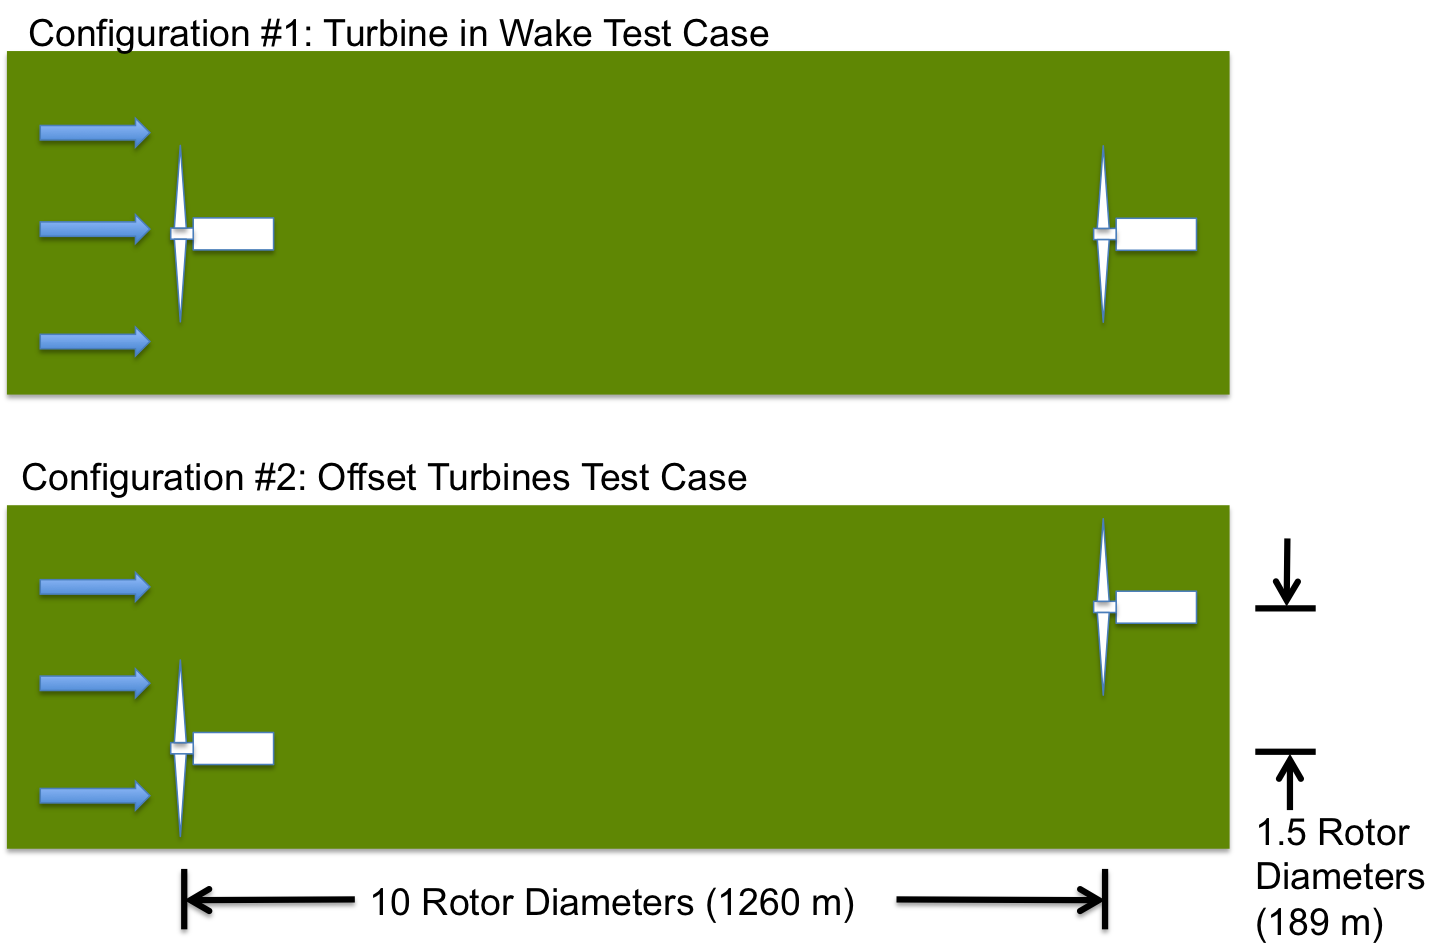
\includegraphics[width = \linewidth]{Figures/ch6Figures/fig6-1.png}
		
	\caption{Configurations for SOWFA simulations of feed forward derating control.}
	\label{fig6-1}
\end{figure}

Choosing a grid resolution is a compromise. A fine grid captures flow behavior that coarse grids doesn't capture. However, using a fine grid has a higher computational cost than a coarse grid, requiring more cores and/or more time to run a simulation. One way to balance simulation detail and computational cost is to make the grid resolution finer in the areas of interest (such as near the turbine rotor) and coarser in areas that are of less interest (such as far from the turbine). Another way is to make the grid resolution as fine as it needs to be, but not making it any finer. 

For simulations in Section \ref{section5-4-1} (referencing a chapter 5 section that hasn't been inserted yet) a grid resolution of 1 meter was used near the turbine rotor. This near-rotor grid was not very large, extending only 1 rotor diameter upstream, 6 rotor diameters downstream, and 1.4 rotor diameters radially, which is approximately 0.04\% of the simulation domain volume. However, this near-rotor grid contains approximately 11 million cells, which is about 57\% of the cells in the simulation domain. A 1 m $\times$ 1 m $\times$ 1 m grid large enough to encompass the two turbine systems shown in figure \ref{fig6-1} would have a prohibitively large number of cells and have a prohibitively high computational cost. 

To make the computational cost more manageable a 2 meter near-rotor grid resolution will be used for simulations in this chapter. Though simulation results will be less detailed, we still have high confidence in the accuracy of the results. As Section \ref{section5-4-3} shows, even a near-rotor grid resolution of 4 meters yielded good agreement for power generation, rotor thrust, wake vorticity, and momentum deficit.  

%----------------------------------------------------------------------------------------
%	SECTION 4
%----------------------------------------------------------------------------------------

\section{Tuning and Validation of SOWFA Turbine \\
		Model} \label{section6-4}

An actuator line model couples SOWFA's LES based atmosphere model to SOWFA's FAST based turbine dynamics model. To get accurate turbine performance from SOWFA, the actuator line model must be tuned. A series of simulations revealed that an actuator line model with 62 elements per blade and a Gausian projection width of 7.5 meters yields good agreement between SOWFA and FAST simulations. These actuator line parameters comply with the best practices recommended by Churchfield, Lee, and Moriarty \cite{churchfield2012} as well as those recommended by Troldborg \cite{troldborg2009}. It is worth noting that the Gausian projection width chosen here is different than the one chosen for SOWFA simulations in Chapter \ref{Chapter5}. This difference is partially due to the use of a 2 meter near-rotor grid resolution, but it is also caused by a difference in tuning requirements. The SOWFA simulations carried out in Chapter \ref{Chapter5} did not model turbine control, so the actuator line was only tuned to produce good agreement on turbine loads and power generation. The Gausian projection width chosen here produces good agreement on controller behavior as well as loading and power generation for wind speeds between 12 and 25 m/s (the range of wind speeds for which the turbine is operating in region 3 control).

To illustrate the close agreement between SOWFA and FAST simulations three simple test cases from chapter 4 are simulated in SOWFA. In these test cases the turbine is subjected to a constant, uniform wind. At 100 seconds the turbine is derated by 20\%. At 200 seconds the turbine is returned to full rated operation. Incoming wind speeds of 12 m/s, 16 m/s, and 20 m/s are simulated. Figures \ref{fig6-2} through \ref{fig6-6} show FAST and SOWFA simulation results for the 16 m/s test case. We see in the figures that FAST and SOWFA produce nearly identical results for rotor speed, power, and blade root bending moments. There is also good agreement on blade pitch and tower base bending moment. SOWFA predicts slightly lower blade pitch angels for this case with a maximum discrepancy of 2.0\% (or 0.25\degree) at 217 seconds. As shown in Figure \ref{fig6-6}, SOWFA predicts more high frequency oscillations in tower base bending moment than FAST. However, there is close agreement on the magnitudes of the predicted loads. 

\begin{figure}[ht]
	\centering
	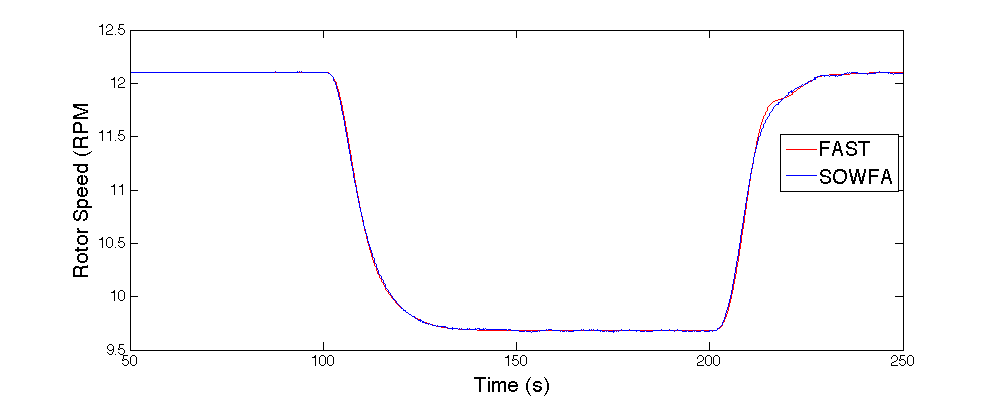
\includegraphics[width = \linewidth]{Figures/ch6Figures/fig6-2.png}		
	\caption{Comparison of rotor speed predicted by FAST and SOWFA for a turbine in 16 m/s winds that is derated by 20\%. }
		\label{fig6-2}
\end{figure}

\begin{figure}[ht]	
	\centering
		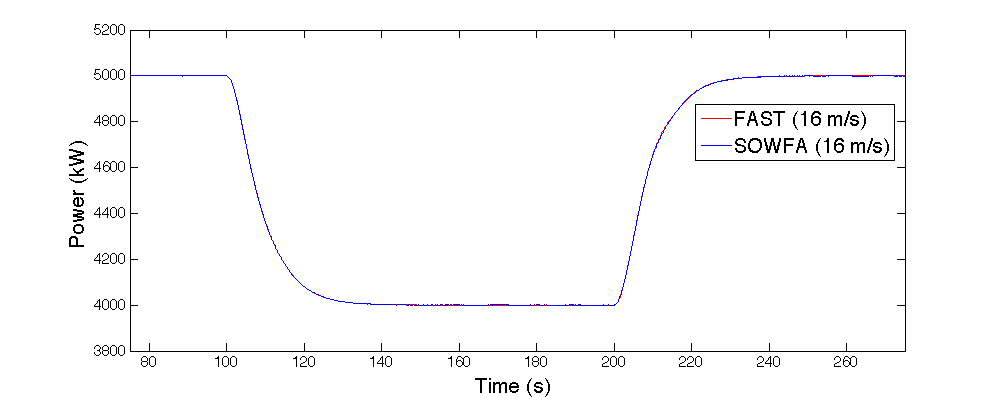
\includegraphics[width = \linewidth]{Figures/ch6Figures/fig6-3.png}
	\caption{Comparison of power predicted by FAST and SOWFA for a turbine in 16 m/s winds that is derated by 20\%.}
	\label{fig6-3}
\end{figure}

\begin{figure}[ht]	
	\centering
		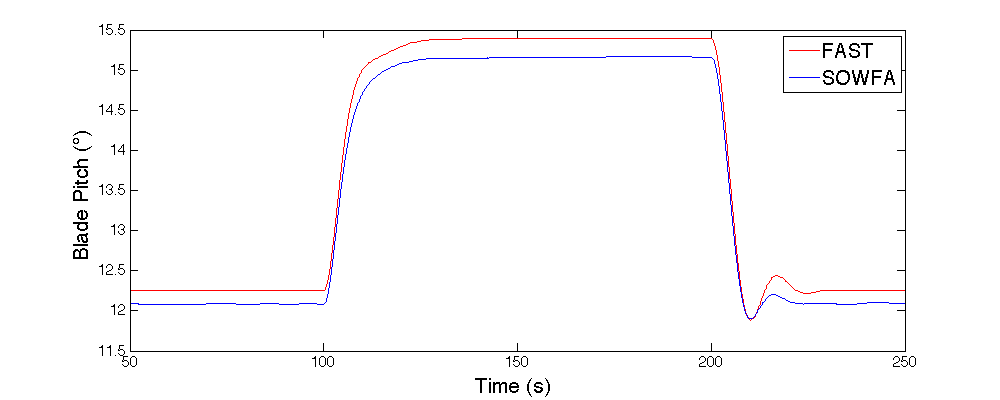
\includegraphics[width = \linewidth]{Figures/ch6Figures/fig6-4.png}

	\caption{Comparison of blade pitch predicted by FAST and SOWFA for a turbine in 16 m/s winds that is derated by 20\%.}
	\label{fig6-4}
\end{figure}

\begin{figure}[ht]	
	\centering
		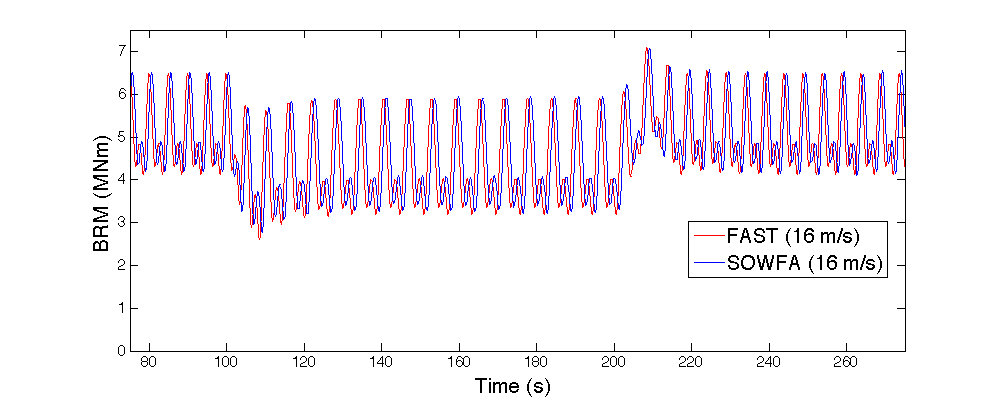
\includegraphics[width = \linewidth]{Figures/ch6Figures/fig6-5.png}

	\caption{Comparison of blade blade root bending moment predicted by FAST and SOWFA for a turbine in 16 m/s winds that is derated by 20\%.}
	\label{fig6-5}
\end{figure}

\begin{figure}[ht]	
	\centering
		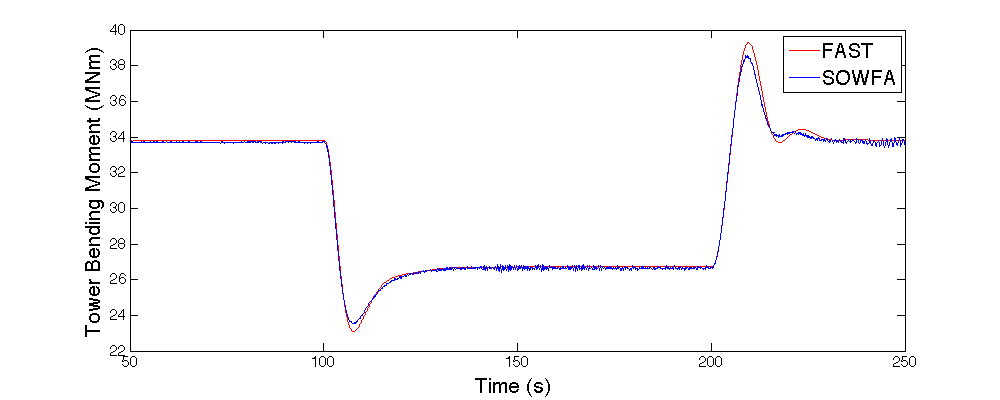
\includegraphics[width = \linewidth]{Figures/ch6Figures/fig6-6.png}

	\caption{Comparison of tower base bending moment predicted by FAST and SOWFA for a turbine in 16 m/s winds that is derated by 20\%.}
	\label{fig6-6}
\end{figure}



Figures \ref{fig6-7} and \ref{fig6-8} show the blade pitch predicted by FAST and SOWFA for the  12 m/s and 20 m/s test cases. For these cases, like the 16 m/s case, FAST and SOWFA had similar predictions for rotor speed, power, and blade root bending moments. We see in Figure \ref{fig6-7} that SOWFA predicts a slightly larger blade pitch when the turbine is operating at full rated capacity in 12 m/s wind. The discrepancy is approximately 0.25\degree . SOWFA also predicts less oscillation in blade pitch following transitions into and out of derated operation. The Despite these discrepancies I still consider this good agreement and evidence of a well tuned SOWFA actuator line model.   



\begin{figure}[ht] 
	\centering
		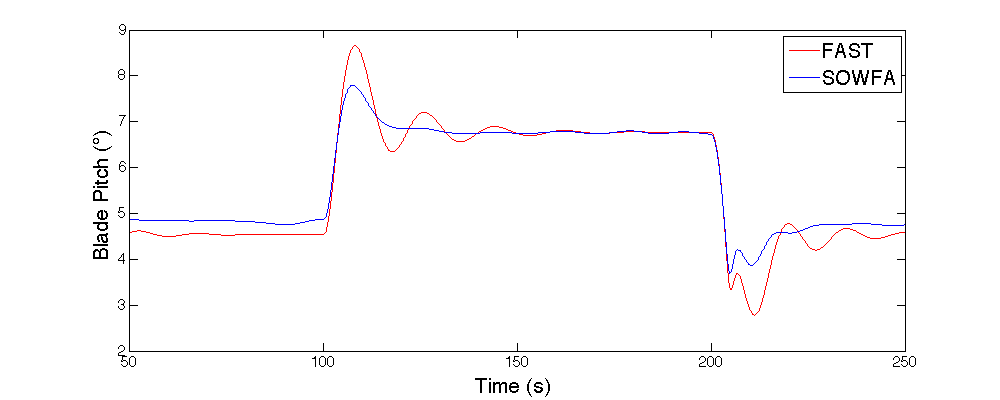
\includegraphics[width = \linewidth]{Figures/ch6Figures/fig6-7.png}

	\caption{Comparison of blade pitch predicted by FAST and SOWFA for a turbine in 12 m/s winds that is derated by 20\%.}
	\label{fig6-7}
\end{figure}

\begin{figure}[ht]	
	\centering
		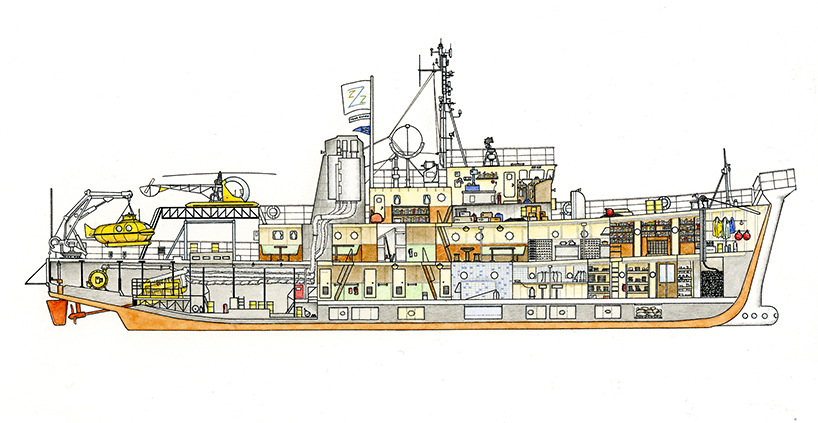
\includegraphics[width = \linewidth]{Figures/ch6Figures/fig6-p.png}

	\caption{Comparison of blade pitch predicted by FAST and SOWFA for a turbine in 20 m/s winds that is derated by 20\%}
	\label{fig6-8}
\end{figure}

%----------------------------------------------------------------------------------------
%	SECTION 5
%----------------------------------------------------------------------------------------

\section{Gust Modeling in SOWFA} \label{section6-5}

For the FAST simulations in Chapter \ref{Chapter4} gusts are modeled by simply increasing the incoming wind speed. However, this method does not work in SOWFA. SOWFA models airflow as an incompressible fluid in a finite computational domain. Increasing the wind speed across the inlet would cause an increase in the amount of air flowing into the computational domain. Because the fluid is incompressible and constrained, conservation of mass dictates that an increase in the amount of air flowing into the domain be immediately matched by an increase in the amount of air flowing out of the domain and an increase in the amount of air flowing from the input to the output. Therefore, increasing the wind speed across the inlet of the computational domain causes an instantaneous increase in wind speed throughout the computational domain.

To model a gust propagating through a wind farm we must be more subtle. This is done by increasing wind speed across part of the inlet, while decreasing wind speed elsewhere in the inlet. As long as the total amount of air flowing into the domain remains the same, the flow far downstream of the inlet will not be affected. Using this method, the gust is localized near the inlet initially then propagates through the computational domain over time. 

In SOWFA, the user can specify a time varying velocity profile across the inlet by applying a TimeVaryingMappedFixedValue boundary condition. For this boundary condition, the user specifies a list of locations on the inlet plane, then specifying velocities at those points for several simulation times. SOWFA interpolates between the supplied data to determine the velocity profile across the inlet for all time steps in the simulation.

Several inlet velocity profiles were investigated in a series of preliminary SOWFA simulations. The inlet profile was found to have a large effect on how the gust initially appears in the simulation domain and how it behaves as it propagates through the domain. Inlet profiles that confine the gust to a small portion of the inlet were found to give the most control over gust behavior. When the gust covers a large portion of the inlet profile, SOWFA smooths out the effect of the gust. This smoothing effect turns rapid velocity changes at the inlet into more gradual velocity changes within the simulation domain. In the following sections we use inlet profiles that confine the gust to a small portion of the inlet. On the remainder of the inlet, the velocity remains constant. 

In chapter \ref{Chapter4} the turbines were subjected to a hat shaped Extreme Operating Gust as defined in section 6.3.2.2 of IEC61400-1\cite{IEC2005}. Preliminary SOWFA simulations found that it is not possible to simulate a hat shaped gust that will propagate through the SOWFA simulations domain. A hat shaped fluctuation of the inlet velocity begins as a hat shaped gust near the inlet. However, the gust decreased in magnitude and changed shape as it moved through the simulation domain. Instead, simulations in the following sections will model an Extreme Coherent Gust similar to the one defined in section 6.3.2.5 of IEC61400-1. 

Figure \ref{fig6-11} illustrates the difference between an Extreme Operating Gust (EOG) and an Extreme Coherent Gust (ECG). The EOG is a brief fluctuation in wind speed, while the ECG is a sustained increase. IEC1400-1 defines the ECG as a 15 m/s increase in wind speed described by equation \ref{eq6-1}. For simulations in this chapter, the 15 m/s ECG magnitude specified by IEC1400-1 is interpreted to be a maximum coherent gust magnitude, not a required magnitude. If a 15 m/s coherent gust is possible then smaller magnitude coherent gusts are also possible. Coherent gusts were found to propagate through the SOWFA simulation domain with only small changes to the magnitude and shape of the gust, as illustrated in figure \ref{fig6-12}



\begin{figure}[ht] 
	\centering
		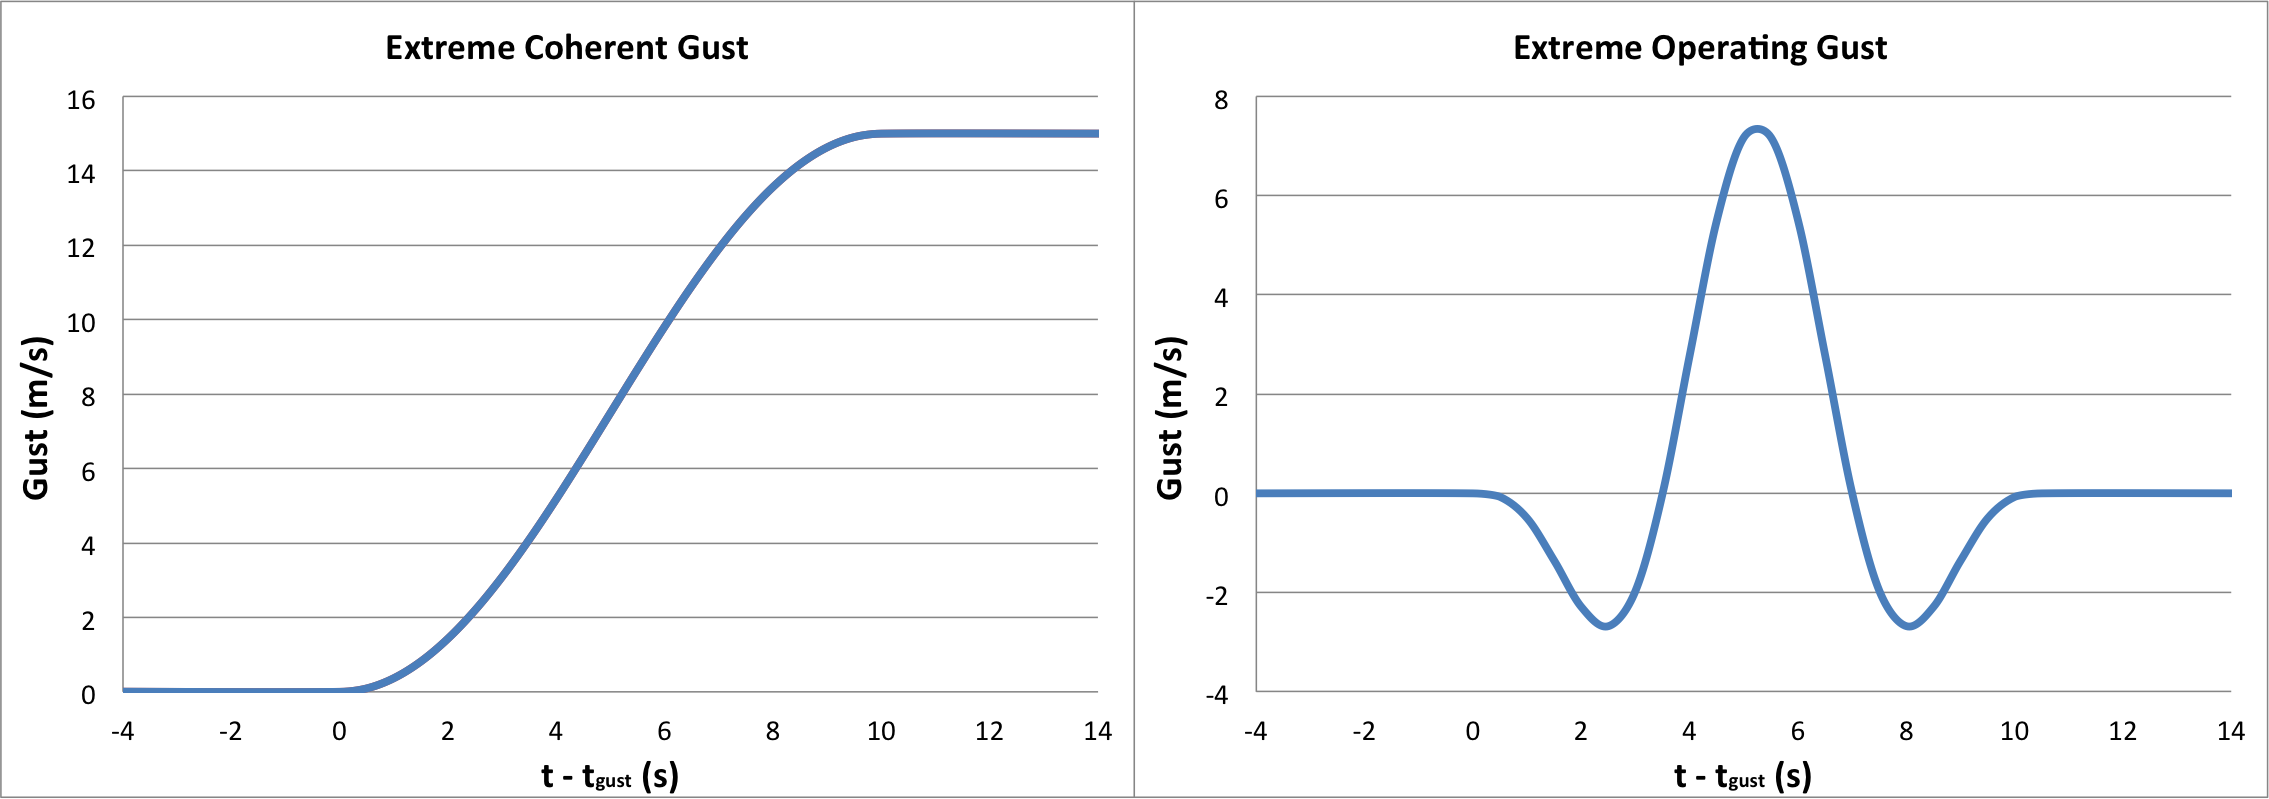
\includegraphics[width = \linewidth]{Figures/ch6Figures/fig6-11.png}

	\caption{Velocity profiles for Extreme Operating Gust (EOG) and Extreme Coherent Gust (ECG).}
	\label{fig6-11}
\end{figure}

\begin{equation} 
	U_{gust}=\left\{\begin{matrix}
0 & for  & t<t_{gust}\\ 
 7.5(1-cos(\pi t/10)) m/s & for  & t_{gust} \leq t<(t_{gust}+10)\\ 
 15 m/s &  for & \leq (t_{gust} +10)
\end{matrix}\right. 
\label{eq6-1}
\end{equation}

\begin{figure}[ht] 
	\centering
		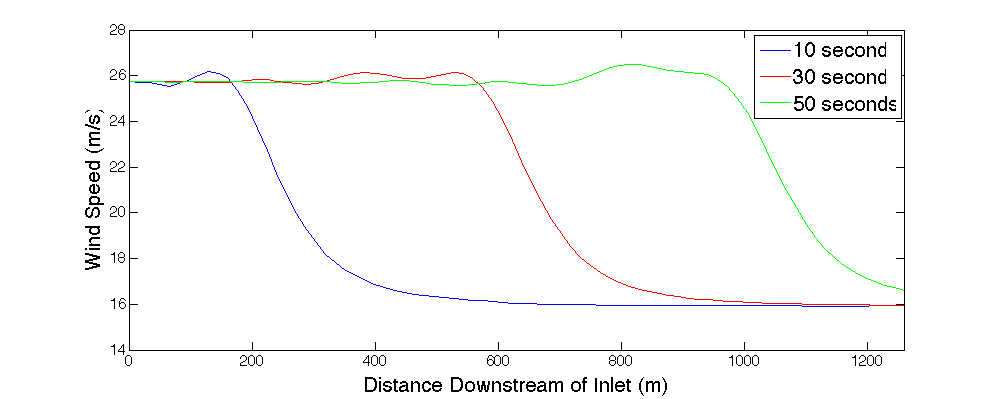
\includegraphics[width = \linewidth]{Figures/ch6Figures/fig6-12.png}

	\caption{Center line velocity as ECG propagates through computational domain.}
	\label{fig6-12}
\end{figure}

%----------------------------------------------------------------------------------------
%	SECTION 6
%----------------------------------------------------------------------------------------
\section{Offset Turbines Test Case} \label{section6-6}

This section documents SOWFA simulations of the offset turbine test case illustrated in figure \ref{fig6-1}. In this test case one turbine is 20R downwind of and 3R to the side of another turbine, where R is the rotor radius of 63 meters. Because of the 3R offset, the downwind turbine is not in the wake of the upwind turbine. This is the configuration that was assumed for FAST simulations of feed forward derating control carried out in Chapter \ref{Chapter4}. 


%-----------------------------------
%	SUBSECTION 6-1
%-----------------------------------
\subsection{Simulation Setup} \label{section6-6-1}

The computational domain is 80R (5,040 m) long, extending 20R in front of the upwind turbine and 40R behind the downwind turbine. The domain is 40R tall, extending 20R above and below the turbine rotors. The domain is also 40R. Each rotor is 38.5R from one side and 41.5R from the other side due to the offset between the upwind and downwind turbine. Initially the domain is constructed of cube shaped cells approximately 32 m $\times$ 32 m $\times$ 32 m, but portions of the domain go through a series of grid refinements to reduce the size of cells to approximately 2 m $\times$ 2 m $\times$ 2 m near the rotors. Table \ref{Table6-1} describes the dimensions and resolutions of each refinement region. The first three refinement regions are rectangular cuboid shaped regions that encompass both turbines. These refinement regions are centered in the computational domain with respect to width and height. In the streamwise direction refinement regions 1, 2, and 3 begin 8.5R, 4.5R, and 2.5R (respectively) in front of the upwind turbine. Refinement regions 4 and 5 are cylindrical in shape and each encompass one of the two turbines. Each of these cylindrical refinement regions is centered on the rotational axis of a turbine rotor, extending 1.5R in front of and 12R behind the rotor.


\begin{table} [ht]
\centering
\begin{tabular}{c c c c c}
\hline
Refinement & Streamwise  & Width & Height & Max Cell Size\\
Region & Length(\emph{R}) & (\emph{R})  &  (\emph{R}) & in Region\\
\hline
1 & 68.5\emph{R} (4316 m)  & 20.2\emph{R} (1272 m) & 17.2\emph{R} (1084 m) & 16 m $\times$ 16 m $\times$ 16 m\\
2 & 64.5\emph{R} (4064 m)  & 12.2\emph{R} (768 m) & 8.2\emph{R} (516 m)  & 8 m $\times$ 8 m $\times$ 8 m\\
3 & 46.5\emph{R} (2930 m)  & 8.2\emph{R} (516 m) & 5.2\emph{R} (328 m)  & 4 m $\times$ 4 m $\times$ 4 m\\
\\
4 \& 5 & 13.5\emph{R} (851 m)    & \multicolumn{2}{c}{Radius = 1.6\emph{R} (101 m)}   & 2 m $\times$ 2 m $\times$ 2 m\\
\hline
\end{tabular}
\caption{ Dimensions and resolutions of the SOWFA grid refinement regions for the Offset Turbines test case.}
\label{Table6-1}
\end{table}

Each simulation is 700 seconds long, but the first 300 seconds are disregarded. This is to ensure that both turbines and their wakes have reached steady state before we start collecting data. Initially the inlet of the computational domain has a uniform 12 m/s wind speed. At 400 seconds a coherent gust is introduced in the center of the computational domain inlet. 

The coherent gust used in the offset turbine test case is 567 m tall $\times$ 756 m wide and is illustrated in Figure \ref{fig6-13}. This is essentially a round gust that has been elongated by 3R (189 m) to ensure it encompasses both turbines. For the part of the gust between the rotor centerlines,  wind speed is given by equation \ref{eq6-2}, where $h_g$ is the distance above or below the rotor centerlines. For the part of the gust to the left or right of the rotor center lines, wind speed is given by equation \ref{eq6-3}, where $r_g$ is the radial distance from the closest rotor centerline. As discussed in Section \ref{section6-5}, the coherent gust contains both higher speed regions (up to 26.16 m/s) and lower speed regions (as low as 5.11 m/s) so the average wind speed across the computational domain inlet remains 12 m/s. For the regions directly upwind of each rotor the average wind speed during the extreme operating gust is 25 m/s, which is the upper limit of the NREL 5-MW turbine operating range. 

\begin{figure}[ht]  
	\centering
		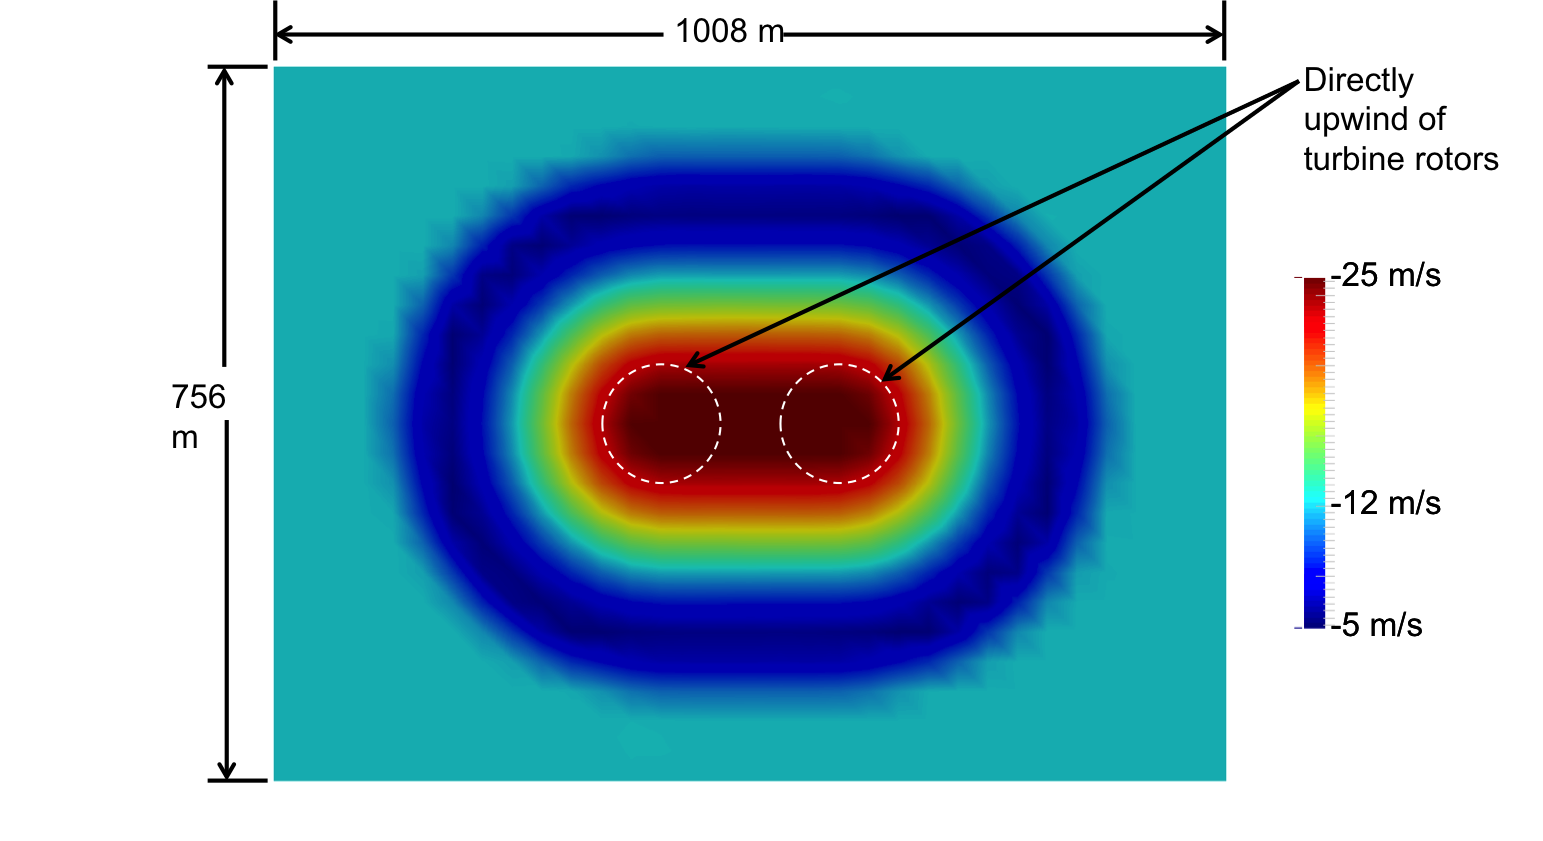
\includegraphics[width = \linewidth]{Figures/ch6Figures/fig6-13.png}

	\caption{Wind speed near center of inlet during Extreme Coherent Gust (offset turbine test case).}
\label{fig6-13}
\end{figure}

\begin{equation} 
	U_{gust}=\left\{\begin{matrix}
\left [15.6312 +10.5248Cos\left ( \frac{h_g}{252 }\pi  \right )  \right ]m/s & for  & h_g<252\\ 
 \left [8.5532 -3.4468Cos\left ( \frac{h_g-252}{31.5}\pi  \right )  \right ]m/s & for  & 252 \leq h_g <283.5\\ 
 12 m/s &  for & 283.5 \leq h_g
\end{matrix}\right. 
\label{eq6-2}
\end{equation}
\begin{equation} 
	U_{gust}=\left\{\begin{matrix}
\left [15.6312 +10.5248Cos\left ( \frac{r_g}{252 }\pi  \right )  \right ]m/s & for  & r_g<252\\ 
 \left [8.5532 -3.4468Cos\left ( \frac{r_g-252}{31.5}\pi  \right )  \right ]m/s & for  & 252 \leq r_g <283.5\\ 
 12 m/s &  for & 283.5 \leq r_g
\end{matrix}\right. 
\label{eq6-3}
\end{equation}

%-----------------------------------
%	SUBSECTION 6-2
%-----------------------------------
This section documents the results of the Offset Turbine test case. This test case was run twice, once without Feed Forward Derating Control enabled and once with Feed forward Derating Control. The following figures and text analyze the behavior of the upwind turbine (which was identical in both runs of the Offset Turbine test case), the behavior of the downwind turbine when Feed Forward Derating Control is not enabled, and the behavior of the downwind turbine when Feed Forward Derating Control is enabled.

Figure \ref{fig6-14} shows wind speed in the computational domain at several key moments when Feed Forward Derating Control is not enabled. Each image in Figure \ref{fig6-14} was generated by taking a horizontal cross section through the center of the computational domain then trimming the cross section to remove regions that were far from the turbines in the downwind or horizontal directions. White lines have been superimposed on the images to show the locations and approximate sizes of the turbine rotors. At t=300 s we see the turbines operating in a steady, uniform 12 m/s wind. The wakes of each turbine are clearly visible, and we see that the downwind turbine is not in the wake of the upwind turbine. At t = 400 s the Extreme Coherent Gust (ECG) enters the computational domain. We see at t = 420 s that the gust has begun to propagate through the domain from left to right. Note that the gust has higher wind speeds at it's center and lower wind speeds near it's edges (as discussed in Section \ref{section6-4}). At t = 480 s we see that the gust has recently reached the upwind turbine. At t = 540 s we see the gust arriving at the downwind turbine. In the t = 540 s image we can also see that there is no wake trailing the upwind turbine. This indicates that the upwind turbine has shut down. At t = 660 s we see that the gust has continued to propagate downstream and there is no wake trailing the downwind turbine, which indicates that it has also shut down. A similar set of images was generated for the Offset Turbine test case with Feed Forward Derating Control (but is not shown here). Those images look very similar, except at t = 600 s. In the t = 600 s image a wake is visible trailing the downwind turbine, which indicates that Feed Forward Derating Control prevents the downwind turbine from shutting down.

 
 \begin{figure}[hp]  
	\centering
		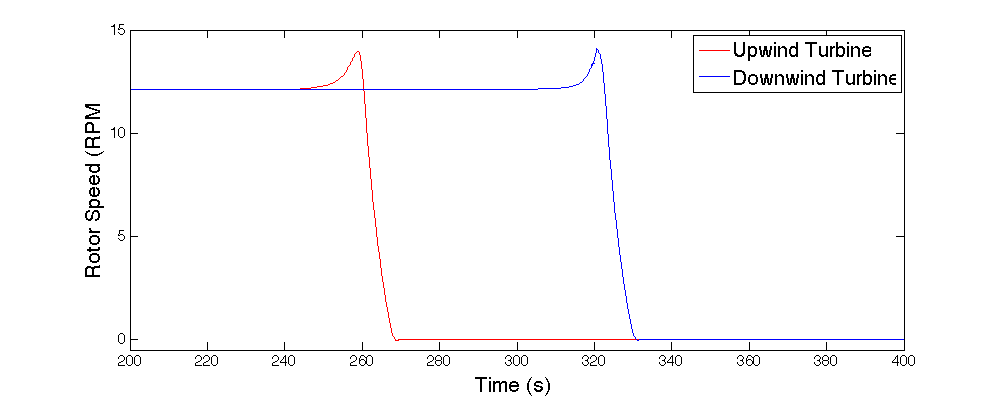
\includegraphics[width = \linewidth]{Figures/ch6Figures/fig6-14.png}

	\caption{Wind speeds at several moments in the Offset Turbines test case without feed forward control.}
	\label{fig6-14}
\end{figure}

It's noteworthy that the gust traveled from the upwind turbine to the downwind turbine in approximately 70 seconds. This corresponds to a convection speed of approximately 18 m/s. For many of the simulations carried out in chapters \ref{Chapter3} and \ref{Chapter4} I assumed Taylor's frozen turbulence hypothesis was valid. I made that assumption because it allowed me to model a two turbine system using FAST, but I noted at the time that the assumption was not expected to be completely valid. If Taylor's frozen turbulence hypothesis was valid for this test case we would expect the gust to propagate downstream at the average domain wind speed of 12 m/s. However, the gust propagates at neither the average wind speed (12 m/s) nor the gust wind speed (~25 m/s), but somewhere in between. This reinforces the importance of using a feed forward control scheme that is tolerant of uncertainty about gust propagation speeds. As discussed in Section \ref{section4-5}, the feed forward selective derating control scheme evaluated in this chapter is highly tolerant of uncertainty in gust propagation speed. The fed forward controller is not required to take any action at the exact moment the gust reaches the downwind turbine. It simply has to derate the turbine some time before the gust arrives and return the turbine to full rated operation some time after the gust has passed.

Figures \ref{fig6-15} through \ref{fig6-19} show the rotor speed, power generation, blade pitch, blade root bending moment, and tower base fore-aft bending moment of the turbines. We see in figures \ref{fig6-15} and \ref{fig6-16} that the turbines have reached steady state operation by t = 300 s. The rotors are turning at a constant rate of 12.1 RPM and  producing 5,000 kW of power. The Extreme Coherent gust reaches the upwind turbine at approximately 450 s, causing both the rotor speed and power generation to increase. At t = 469.7 s the rotor speed exceeds the 15\% overspeed limit and an emergency overspeed shutdown is initiated. If Feed Forward Derating Control is enabled, a signal is sent to the downwind turbine instructing it to derate by 10.37\% beginning at t = 481.7 s and return to full rated operation at t = 627.2 s. The upwind rotor comes to a halt at t = 480.9 s and is stationary for the remaining 219.1 seconds of the simulation. In real world operation this turbine would remain stationary until an operator can verify that is safe to return the turbine to operation. This could potentially be much longer than 219.1 seconds. Between t = 481.7 s and t = 511.7 s the downwind turbine with feed forward control smoothly reduces it's rotor speed and power generation, while the turbine without feed forward control continues to operate at a rotor speed of 12.1 RPM and power generation of 5,000 kW. The Extreme Coherent Gust reaches the downwind turbine at approximately 520 s, causing both the rotor speed and power generation to increase. The downwind turbine without feed forward control exceeds the 15\% overspeed limit at t = 539.2 s and an emergency overspeed shutdown is initiated. By t = 550.5 s the downwind turbine without feed forward control is shut down. The downwind turbine with Feed Forward Derating Control experiences a maximum overspeed of 6.9\%, which does not cause an emergency overspeed shutdown. Between t = 627.2 s and t = 657.2 s the turbine transitions back to full rated operation.

\begin{figure}[ht] 
	\centering
		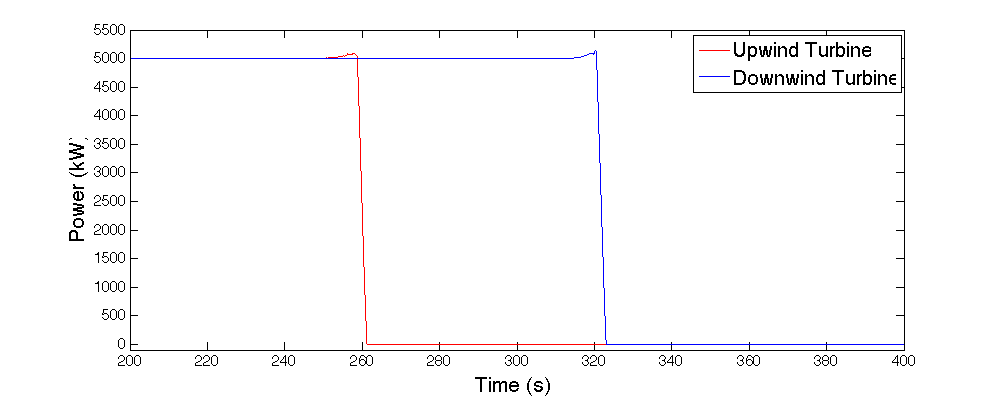
\includegraphics[width = \linewidth]{Figures/ch6Figures/fig6-15.png}

	\caption{Rotor speed during the Offset Turbines test case without feed forward control.}
\end{figure}
\begin{figure}[ht] \label{fig6-16}
	\centering
		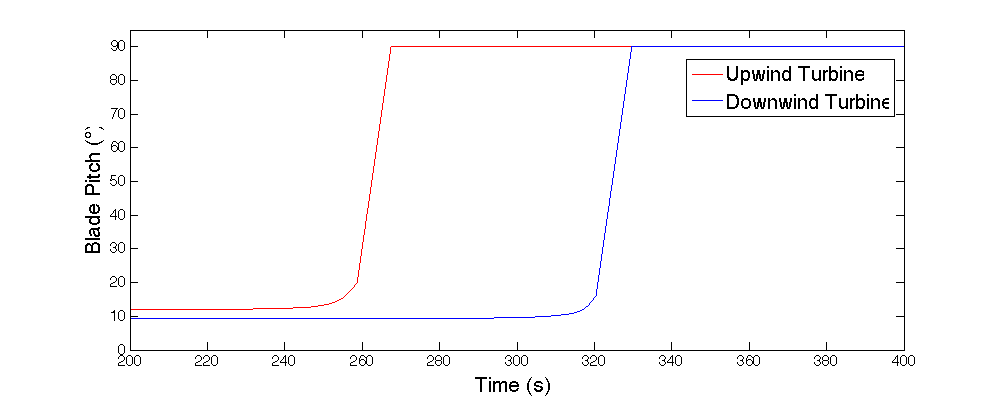
\includegraphics[width = \linewidth]{Figures/ch6Figures/fig6-16.png}

	\caption{Power generation during the Offset Turbines test case without feed forward control.}
	\label{fig6-15}
\end{figure}

Figure \ref{fig6-17} shows the blade pitch of the turbines. Initially, when the turbines are operating in uniform 12 m/s wind, the turbines have a steady blade pitch of 4.8\degree. As the upwind turbine begins to experience increased wind speed it's blade pitch increases. This is an effort by the turbine pitch controller to maintain a constant rotational speed of 12.1 RPM. We see in Figure \ref{fig6-17} the upwind turbine has a blade pitch of 18.3\degree when the emergency shutdown procedure is initiated at t = 469.7 s. After the emergency shutdown is initiated blade pitch increases to 90\degree at a rate of 8\degree /s. The downwind turbine without feed forward control shows similar behavior, reaching a blade pitch of 20.3\degree before the emergency shutdown is initiated at t = 539.2 s. The downwind turbine with Feed Forward Derating Control increases blade pitch from 4.8\degree to 6.1\degree when the turbine is derated (starting at t = 481.7 s). The gust causes an increase and some oscillation in blade pitch, with the blade pitch eventually settling to approximately 25.5\degree. When the turbine is returned to full rated operation, starting at t = 627.2 s, blade pitch decreases to 23.1\degree.

\begin{figure}[ht] 
	\centering
		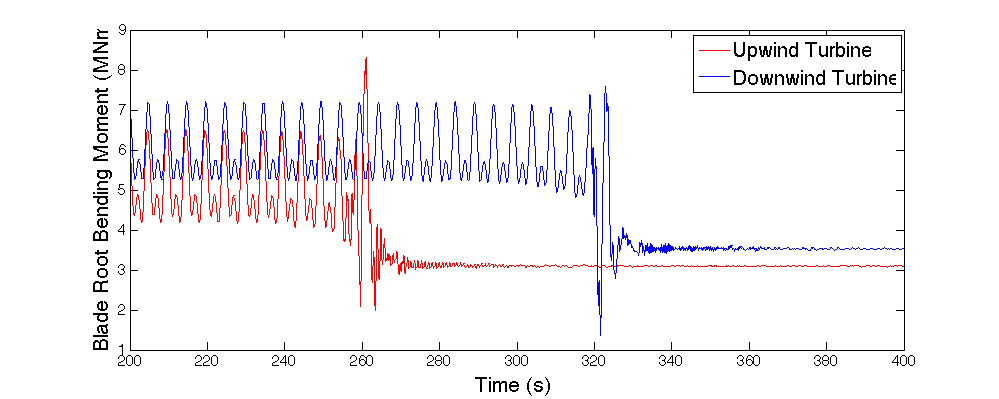
\includegraphics[width = \linewidth]{Figures/ch6Figures/fig6-17.png}

	\caption{Blade pitch during the Offset Turbines test case without feed forward control.}
	\label{fig6-17}
\end{figure}

Figures \ref{fig6-18} shows blade root bending moment (BRM). Initially, when the turbines are operating in uniform 12 m/s wind the blade root bending moment is very regular. The upwind and downwind turbines experience nearly identical cyclical loading. When the upwind turbine begin to experience higher wind speeds and blade pitch begins to increase, the BRM loading cycle maintains it's shape but begins to decrease in magnitude. This effect can be seen from t = 430 s to t = 465 s. During the emergency shutdown process the shape of the BRM loading cycle changes and larger fluctuations in BRM can be seen. When the rotor comes to a halt the BRM settles to a constant value. Note that BRM is not 0 MNm when the turbine rotor stops. This residual loading is due to gravitational loads. BRM would only be 0 MNm if this blade happened to stop pointing directly up or down. The downwind turbine without feed forward control shows similar behavior in response to the Extreme Coherent Gust (EOG) and subsequent shutdown. The BRM loading cycle maintains it's shape but begins to decrease in magnitude between t = 500 s and t = 535 s. The shape of the BRM loading cycle then becomes irregular and there are a few large fluctuations before BRM settles to a constant value. The downwind turbine with Feed Forward Derating Control experiences a 12\% decrease in mean BRM and a 9\% decrease in the magnitude of BRM fluctuations starting at t = 481.7 s. These changes are primarily due to the increase in blade pitch caused by derating. When the Extreme Coherent Gust arrives and blade pitch is increased further, the mean BRM decreases to approximately 3 MNm (~60\% below the initial mean BRM) and the cyclical fluctuations in BRM have increased to approximately 4 MNm (~140\% above the initial magnitude of fluctuations).


\begin{figure}[ht] 
	\centering
		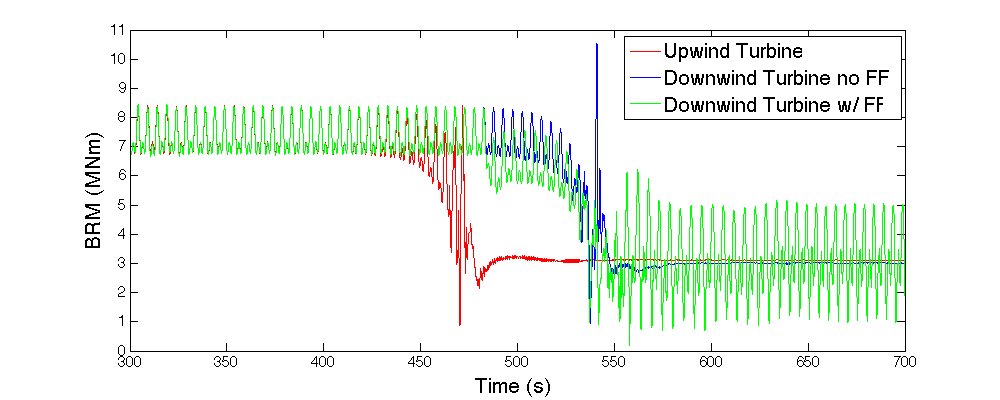
\includegraphics[width = \linewidth]{Figures/ch6Figures/fig6-18.png}

	\caption{Blade root bending moment (BRM) during the Offset Turbines test case without feed forward control.}
	\label{fig6-18}
\end{figure}


In Figure \ref{fig6-19} we see that the upwind turbine and the downwind turbine without feed forward control exhibit similar behavior. Tower base fore-aft bending moments is initially constant at approximately 48 MNm. The tower base bending moment is highly dependent on the aerodynamic loading, which is highly dependent on blade pitch. As wind speeds begin to increase and blade pitches begin to increase we see a smooth reduction in tower fore-aft bending moment. The emergency shutdown process introduces a lot more oscillation in the tower base fore-aft bending moment, including one very large loading cycle where loading goes from approximately 35 MNm to approximately -40 MNm. This large spike in negative loading moment corresponds to the tower swinging forward after the aerodynamic loading on the rotor is suddenly reduced to zero when the blades pitch to 90\degree. Eventually all of the high frequency oscillations in loading die out and the tower base fore-aft bending moment settles to 0 MNm. The downwind turbine with Feed Forward Derating Control also begins with a tower base fore-aft bending moment of 48 MNm, but experiences a reduction in loading when the turbine is derated (starting at t = 481.7 s). This is consistent with a reduction in aerodynamic loading on the turbine rotor due to increasing blade pitch. When the Extreme Coherent Gust arrives the downwind turbine sees a further reduction in the average tower base fore-aft bending moment. However, we see the introduction of a cyclic loading component that persists through the end of the simulation. If we zoom in on these high frequency oscillations we see that the loading has a very similar shape to the cyclic BRM loading seen in Figure \ref{fig6-18}, but has a frequency three times higher. Since the turbine rotor has three blades, this indicates that the higher magnitude BRM oscillations seen near the end of the simulation are causing the high frequency oscillations in tower loading. 



\begin{figure}[ht] 
	\centering
		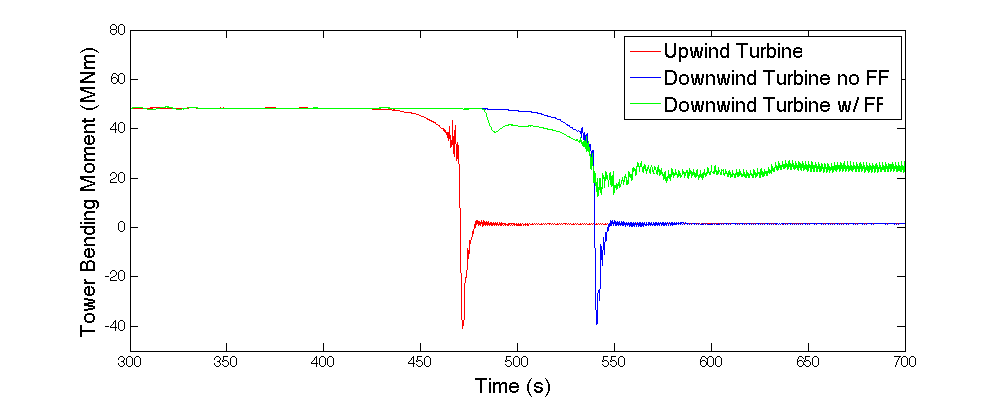
\includegraphics[width = \linewidth]{Figures/ch6Figures/fig6-19.png}

	\caption{Tower base fore-aft bending moment during the Offset Turbines test case without feed forward control.}
	\label{fig6-19}
\end{figure}

Table \ref{Table6-2} summarizes several important performance metrics for the turbines. We see in the table that Feed Forward Derating Control improves turbine behavior in all four performance metrics. The upwind turbine and the downwind turbine without feed forward control have very similar tower base fore-aft bending moment Damage Equivalent Loads (DEL). Feed Forward Derating Control reduces tower base fore-aft bending moment DEL by 44.2 MNm, which is a reduction of 59\%. This is likely because the downwind turbine with feed forward derating control does not experience the very large magnitude loading cycles observed during emergency shutdown. The downwind turbine without feed forward control experiences approximately 20\% higher blade root bending moment (BRM) DEL than the upwind turbine. 

Part of this difference is because the downwind turbine operates for longer and experiences more BRM loading cycles before the gust arrives. A contributing factor may also be the differences in the loading patterns observed near shutdown in Figure \ref{fig6-18}. These differences in loading patterns are caused by the interaction of the loading induced by the Extreme Coherent Gust and the cyclic loading due to the rotation of the turbine rotor. Feed Forward Derating Control reduces DEL BRM by 15\% despite the turbine operating for a longer period of time and enduring a larger quantity of BRM loading cycles. The upwind turbine and the downwind turbine without feed forward control experience similar maximum overspeeds, while the downwind turbine with Feed Forward Derating Control has a significantly smaller maximum overspeed. Finally, we see that the downwind turbine without feed forward control produces 96.46 KWh more energy than the upwind turbine. This is simply because the gust arrives at the downwind turbine ~70 seconds after it arrives at the upwind turbine. This allows the downwind turbine without feed forward control to generate electricity for an additional 70 seconds before experiencing an emergency overspeed shutdown. Feed Forward Derating Control further increases energy generation by 201.27 KWh.




\begin{table} [ht]
\centering
\begin{tabular}{c|cccccccccc}
\hline
\hline
                                                                                         &  & \begin{tabular}[c]{@{}c@{}}Tower Base\\ DEL(MNm)\end{tabular} & & \begin{tabular}[c]{@{}c@{}}Blade Root\\ DEL(MNm)\end{tabular} &  & \begin{tabular}[c]{@{}c@{}}Max\\ Overspeed(\%)\end{tabular} &  &  \begin{tabular}[c]{@{}c@{}}Energy\\ Gen.(kWh)\end{tabular}\\ 
\hline
\begin{tabular}[c]{@{}c@{}}Upwind \\ Turbine \end{tabular}                               &  & 76.4                                                          & & 7.60                                                          &  & 15.37                                 				       &  &  237.54                                                    \\
\\
\begin{tabular}[c]{@{}c@{}}Downwind \\ Turbine \\ Without FF \\ Control\end{tabular}     &  & 75.2                                                          & & 9.15                                                          &  & 15.04                                                       &  &  334.00                                                    \\
\\
\begin{tabular}[c]{@{}c@{}}Downwind \\ Turbine \\ With FF \\ Control \end{tabular}       &  & 31.0                                                          & & 7.82                                                          &  & 6.90                                                        &  &  535.27                                                    \\
\\
\begin{tabular}[c]{@{}c@{}}Change   \\ Due to FF \\ Control          \end{tabular}       &  & \begin{tabular}[c]{@{}c@{}}-44.2 \\ (-58.8\%)  \end{tabular}   & & \begin{tabular}[c]{@{}c@{}} -1.33 \\ (-14.5\%)  \end{tabular}   &  & \begin{tabular}[c]{@{}c@{}} -8.14 \\    \end{tabular}        &  &  \begin{tabular}[c]{@{}c@{}}+201.27\\(+60.2\%)\end{tabular} \\
\\
\hline
\hline                             
\end{tabular}
\caption{Summary of turbine performance metrics and the effects of Feed Forward Derating Control for the Offset Turbine test case.}
\label{Table6-2}
\end{table}


It is important to note that the difference in energy generation could be much larger in real world operation. These simulations end at t = 700 s, but beyond that time the downwind turbine with Feed Forward Derating Control would continue to generate 5 MW (or ~1.4 KWH per second). The downwind turbine without feed forward control would not generate any power until it was returned to service. That turbine may be shut down for much longer than the 149.5 seconds captured in these simulations.

%----------------------------------------------------------------------------------------
%	SECTION 7
%----------------------------------------------------------------------------------------
\section{Turbine in Wake Test Case} \label{section6-7}

In previous chapters we assumed the downwind turbine would be slightly offset from the upwind turbine and would not be in that turbine's wake. This was done out of necessity because FAST is not capable of modelling turbine wake effects. However, SOWFA is well suited to model turbine wakes and how those wakes effect downwind turbines. Mathew Churchfield and others at NREL have published several articles that use SOWFA to study such effects \cite{fleming2014,martinez2015,churchfield2015,lee2012}. Furthermore, wake effects are common in real world wind farms. This section documents SOWFA simulations of the turbine in wake test case illustrated in figure \ref{fig6-1}. In this test case one turbine is 1260 m (or 20R, where R is the rotor radius) directly behind and in the wake of another turbine.

%-----------------------------------
%	SUBSECTION 7-1
%-----------------------------------
\subsection{Simulation Setup} \label{section6-7-1}

The simulation domain is 5040 m $\times$ 2520 m $\times$ 2520 m (or 80R $\times$ 40R $\times$ 40R). This domain extends 1260 m (20R) in front of the upwind rotor and 2520 m (40R) behind the downwind rotor, as well as 1260 m (20R) both horizontally and vertically from the centers of the rotors. The computational domain is initially composed of approximately 32 m $\times$ 32 m $\times$ 32 m cells, but portions of the domain go through a series of grid refinements to reduce the size of the cells near the turbine rotors. The refinement regions are a series of 4 concentric cylinders with centerlines laying on the rotational axis of the NREL 5-MW rotors and having the dimensions shown in Table \ref{Table6-1}. These refinement regions have the same radial dimensions as refinement regions 1 through 4 used in Chapter \ref{Chapter5} SOWFA simulations (Table \ref{Table5-1}). However, the streamwise dimensions have been increased to accommodate a second turbine. In the streamwise direction refinement regions 1, 2, 3, and 4 begin 8.5R, 4.5R, 2.5R, and 1.5R (respectively) in front of the upwind turbine.

\begin{table}[ht]
\centering
\begin{tabular}{c c c c c}
\hline
Refinement & Streamwise       & Radius     & Max Cell Size\\
Region     & Length(\emph{R}) & (\emph{R}) &  in Region\\
\hline
1          & 68.5\emph{R} (4316 m)  & 8.6\emph{R} (542 m) & 16 m $\times$ 16 m $\times$ 16 m\\
2          & 64.5\emph{R} (4064 m   & 4.6\emph{R} (290 m) & 8 m $\times$ 8 m $\times$ 8 m\\
3          & 46.5\emph{R} (2390 m)  & 2.6\emph{R} (164 m) & 4 m $\times$ 4 m $\times$ 4 m\\
4          & 33.5\emph{R} (2111 m)  & 1.6\emph{R} (101 m) & 2 m $\times$ 2 m $\times$ 2 m\\
\hline
\end{tabular}
\caption{ Extents and resolutions of the SOWFA grid refinement regions for the Turbine in Wake test case.}
 \label{Table6-5}
\end{table}

Each simulation is 700 seconds long, but the first 300 seconds are disregarded. This is to ensure that both turbines and their wakes have reached steady state before we start collecting data. Initially the inlet of the computational domain has a uniform 12 m/s wind speed. At 400 seconds a coherent gust is introduced in the center of the computational domain inlet. 

The coherent gust used for the turbine in wake test case is illustrated in Figure \ref{fig6-26} and is described by equation \ref{eq6-4}, where $r_g$ is the radial distance from the centerline of the turbine rotors. As discussed in Section \ref{section6-5}, the coherent gust contains both higher speed regions (up to 26.41 m/s) and lower speed regions (as low as 7.59 m/s) so the average wind speed across the computational domain inlet remains 12 m/s. For the regions directly upwind of the turbine rotors the average wind speed during the extreme operating gust is 25 m/s, which is the upper limit of the NREL 5-MW turbine operating range. 

\begin{figure}[ht] 
	\centering
		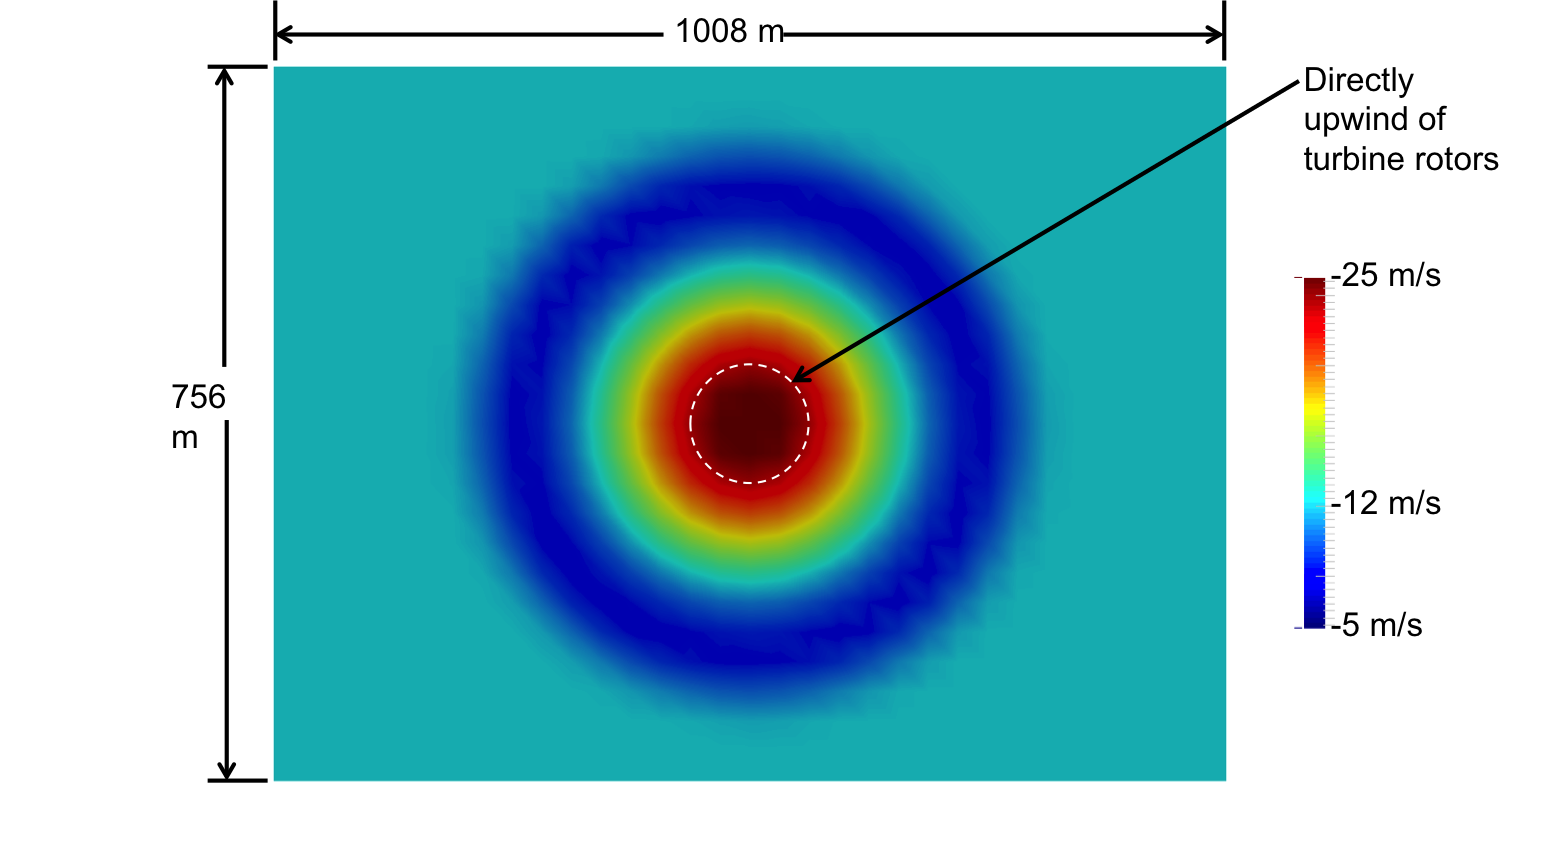
\includegraphics[width = \linewidth]{Figures/ch6Figures/fig6-26.png}

	\caption{Wind speed near center of inlet during Extreme Coherent Gust (Turbine in Wake test case).}
	\label{fig6-26} 
\end{figure}

\begin{equation} 
	U_{gust}=\left\{\begin{matrix}
\left [16.9991 +9.4109Cos\left ( \frac{r_g}{252 }\pi  \right )  \right ]m/s & for  & r_g<252\\ 
 \left [9.794 -2.2060Cos\left ( \frac{r_g-252}{63}\pi  \right )  \right ]m/s & for  & 252 \leq r_g <315\\ 
 12 m/s &  for & 315 \leq r_g
\end{matrix}\right. 
\label{eq6-4}
\end{equation}

%-----------------------------------
%	SUBSECTION 7-2
%-----------------------------------
\subsection{Performance Without Feed Forward Derating Control} \label{section6-7-2}

This section documents the results of the Turbine in Wake test case. This test case was run twice, once without Feed Forward Derating Control enabled and once with Feed forward Derating Control. The following figures and text analyze the behavior of the upwind turbine (which was identical in both runs of the Offset Turbine test case), the behavior of the downwind turbine when Feed Forward Derating Control is not enabled, and the behavior of the downwind turbine when Feed Forward Derating Control is enabled.

Figure \ref{fig6-27} shows wind speed in the computational domain at several key moments when Feed Forward Derating Control is not enabled. Each image in Figure \ref{fig6-14} was generated by taking a horizontal cross section through the center of the computational domain then trimming the cross section to remove regions that were far from the turbines in the downwind or horizontal directions. White lines have been superimposed on the images to show the locations and approximate sizes of the turbine rotors. At t=300 s we see that the upwind turbine is operating in a steady, uniform 12 m/s wind. The downwind turbine is subject to a lower and less consistent wind speed because it is in the wake of the upwind turbine. At t = 400 s the Extreme Coherent Gust enters the computational domain. We see at t = 420 s that the gust has begun to propagate through the domain from left to right. At t = 480 s we see that the gust has recently reached the upwind turbine. At t = 540 s we see the gust arriving at the downwind turbine. In the t = 540 s image we can also see that there is no wake trailing the upwind turbine. This indicates that the upwind turbine has shut down. At t = 660 s we see that the gust has continued to propagate downstream and there is no wake trailing the downwind turbine, which indicates that it has also shut down. A similar set of images was generated for the Turbine in Wake test case with Feed Forward Derating Control (but is not shown here). Those images look very similar, except at t = 600 s. In the t = 600 s image a wake is visible trailing the downwind turbine, which indicates that Feed Forward Derating Control prevents the downwind turbine from shutting down.

 \begin{figure}[hp] 
	\centering
		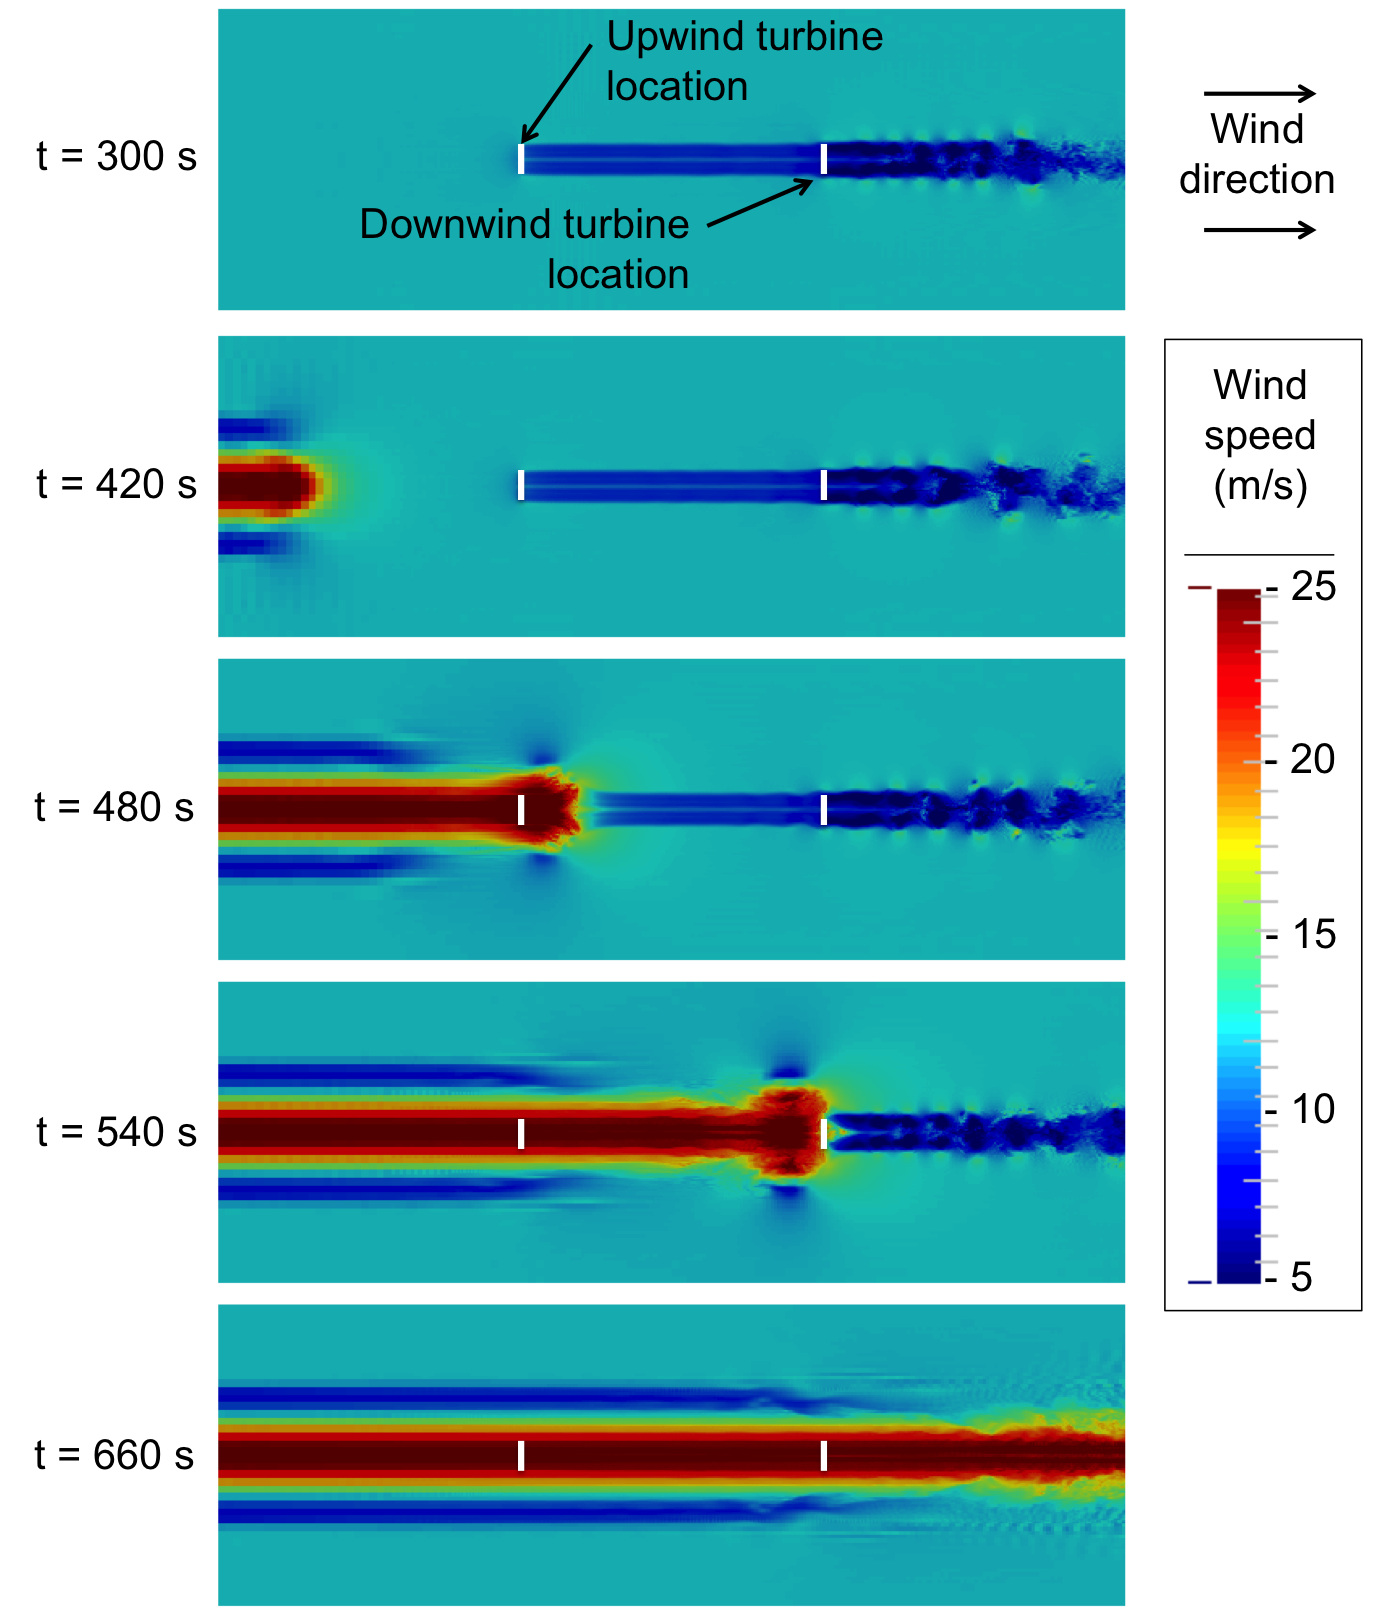
\includegraphics[width = \linewidth]{Figures/ch6Figures/fig6-27.png}

	\caption{Wind speeds at several moments for the Turbine in Wake test case without feed forward control.}
	\label{fig6-27} 
\end{figure}

 Figures \ref{fig6-28} through \ref{fig6-32} show the rotor speed, power generation, blade pitch, blade root bending moment, and tower base fore-aft bending moment of the turbines. In Figure \ref{fig6-28} we see that the upwind turbine is initially rotating at a constant rate of 12.1 RPM. This is expected for a turbine in 12 m/s wind because it is operating in region 3 control. The downwind turbine, which is in the wake of the upwind turbine,  has a lower rotational speed with some fluctuations. The lower rotational speed indicates that the downwind turbine is operating in region 2 control, which does not track a constant rotational speed. Region 2 control uses generator torque to vary rotational speed in an attempt to maximize power generation. The Extreme Coherent gust reaches the upwind turbine at approximately t = 450 s, triggering an emergency overspeed shutdown at t = 466.7 s. If Feed Forward Derating Control is enabled, a signal is sent to the downwind turbine instructing it to derate by 11.12\% beginning at t = 478.7 s and return to full rated operation at t = 624.2 s. Between t = 478.7 s and t = 508.7 s the downwind turbine with Feed Forward Derate Control smoothly reduces it's rotor speed and power generation, while the downwind turbine without feed forward control continues to operate according to normal region 2 control. The Extreme Coherent Gust reaches the downwind turbine at approximately t = 520 s. The downwind turbine without feed forward control exceeds the 15\% overspeed limit at t = 538.6 s and an emergency overspeed shutdown is initiated. The downwind turbine with Feed Forward Derate Control experiences a maximum overspeed of 11.12\% , which does not cause an emergency overspeed shutdown. Between t = 624.2 s and t = 654.2 s the downwind turbine transitions back to full rated operation.


 Figures \ref{fig6-28} through \ref{fig6-32} show the rotor speed, power generation, blade pitch, blade root bending moment, and tower base fore-aft bending moment of the turbines. We see in figures \ref{fig6-28} and \ref{fig6-29} that the upwind turbine is initially rotating at a constant rate of 12.1 RPM and producing 5,000 kW of power. This is expected for a turbine in 12 m/s wind because it is operating in region 3 control. The downwind turbine, which is in the wake of the upwind turbine,  has a lower rotational speed and a lower power generation. The downwind turbine also has some fluctuations in rotor speed and power generation. The lower rotational speed indicates that the downwind turbine is operating in region 2 control, which does not track a constant rotational speed. Region 2 control uses generator torque to vary rotational speed in an attempt to maximize power generation. The Extreme Coherent gust reaches the upwind turbine at approximately t = 450 s, triggering an emergency overspeed shutdown at t = 466.7 s. If Feed Forward Derating Control is enabled, a signal is sent to the downwind turbine instructing it to derate by 11.12\% beginning at t = 478.7 s and return to full rated operation at t = 624.2 s. Between t = 478.7 s and t = 508.7 s the downwind turbine with Feed Forward Derate Control smoothly reduces it's rotor speed and power generation, while the downwind turbine without feed forward control continues to operate according to normal region 2 control. The Extreme Coherent Gust reaches the downwind turbine at approximately t = 520 s. The downwind turbine without feed forward control experiences a large spike in rotor speed and power generation (a much larger change than what the upwind turbine experiences) as it is briefly put into region 3 operation. At t = 538.6 s the downwind turbine without feed forward control exceeds the 15\% overspeed limit and an emergency overspeed shutdown is initiated. The downwind turbine with Feed Forward Derate Control experiences a maximum overspeed of 11.12\% , which does not cause an emergency overspeed shutdown. Between t = 624.2 s and t = 654.2 s the downwind turbine transitions back to full rated operation.

\begin{figure}[ht] 
	\centering
		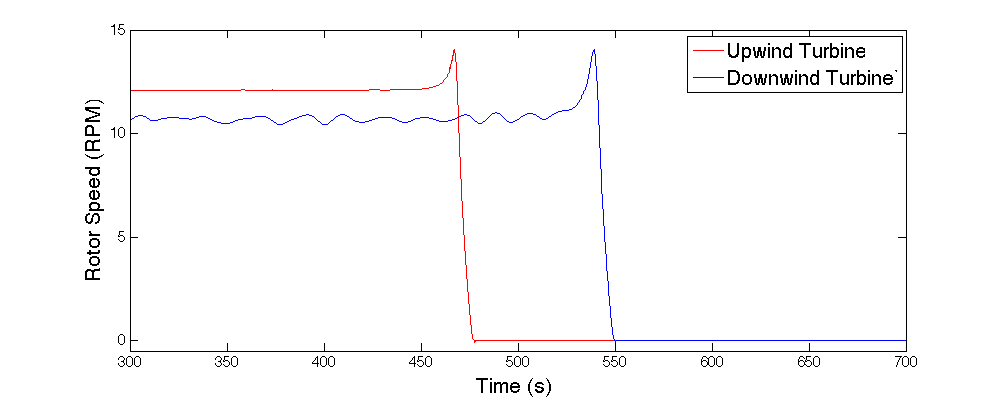
\includegraphics[width = \linewidth]{Figures/ch6Figures/fig6-28.png}
	\caption{Rotor speed during the Turbine in Wake test case without feed forward control.}
	\label{fig6-28}
\end{figure}

\begin{figure}[ht] 
	\centering
		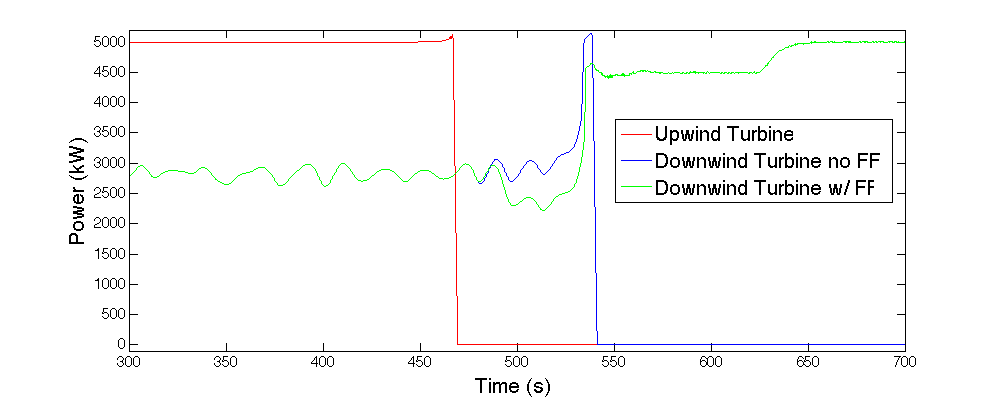
\includegraphics[width = \linewidth]{Figures/ch6Figures/fig6-29.png}

	\caption{Power generation during the Turbine in Wake test case without feed forward control.}
	\label{fig6-29}
\end{figure}

On average the downwind turbine is producing approximately 2800 kW of power prior to the Extreme Coherent Gust. This is 44\% less power than the upwind turbine, which illustrates that wake effects can have a very large impact on power production.The downwind power generation seen in Figure \ref{fig6-27} is consistent with the rotor speeds seen in Figure \ref{fig6-28}, is consistent with results in Chapter \ref{Chapter4}, and is consistent with results that other researchers have published for wake effects 20R downstream of a turbine in turbulence free conditions. For an NREL 5-MW turbine, power production of 2800 kW corresponds to an effective incoming wind speed of 9.4 m/s. This indicates that the upwind turbine wake is causing an average wind velocity deficit of 22\%  at the downwind turbine (20R downstream).This is similar to the velocity deficit shown in Figure \ref{fig5-5}-b. A 22\% wind velocity deficit is also consistent with the findings of Troldborg et al. for RANS (Reynolds Averaged Navier Stokes) simulations of an NREL 5-MW turbine \cite{troldborg2015}, and LES (Large Eddy Simulation) based simulations of a 2MW NEG Micon NM80 turbine \cite{troldborg2010,troldborg2010b}. Furthermore, a 22\% wind velocity deficit is consistent with the dynamic wake meandering model described by Madsen et al. \cite{madsen2010}. These publications looked at a variety of turbine operating conditions and several noteworthy trends were found. Velocity deficit decreases as downstream distance increases. Velocity deficits decrease faster in turbulent conditions than in turbulence free conditions. Velocity deficits are largest when the turbine is in region 2 operation. When in region 3 operation, velocity deficit decreases as wind speed increases.


Figure \ref{fig6-30} shows the blade pitch of the turbines. Initially, the upwind turbine has a blade pitch of 4.8\degree and the downwind turbine has a pitch of 0\degree. As the upwind turbine begins to experience increased wind speed (at t = ~450 s) it's blade pitch increases in an effort to maintain a constant rotational speed of 12.1 RPM. The upwind turbine's blade pitch is at 15.3\degree when the emergency shutdown procedure is initiated at t = 466.7 s. After the emergency shutdown is initiated blade pitch increases to 90\degree at a rate of 8\degree /s. The downwind turbine begins to experience increased wind speed at t = ~520 s. The downwind turbine without feed forward control maintains a blade pitch of 0\degree until the rotor speed increases to 12.1 RPM. Once the rotor speed reaches 12.1 RPM the turbine transitions from region 2 control to region 3 control and increases blade pitch in an effort to maintain that rotational speed. The upwind turbine's blade pitch is at 10.4\degree when the emergency shutdown procedure is initiated at t = 538.6 s. The downwind turbine with Feed Forward Derating Control increases blade pitch from 0\degree to 2.6\degree when the turbine is derated (starting at t = 478.7 s). The gust causes an increase and some oscillation in blade pitch, with the blade pitch eventually settling to approximately 25.5\degree. When the turbine is returned to full rated operation, starting at t = 624.2 s, blade pitch decreases to 23.1\degree.

As the downwind turbine without feed forward control begins to experience increased wind speed (at t = ~520 s) the turbine 

\begin{figure}[ht] 
	\centering
		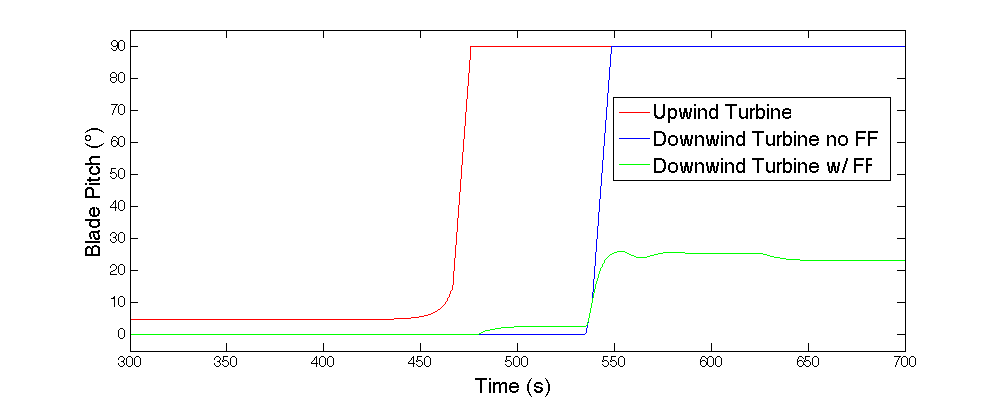
\includegraphics[width = \linewidth]{Figures/ch6Figures/fig6-30.png}

	\caption{Blade pitch during the Turbine in Wake test case without feed forward control.}
	\label{fig6-30}
\end{figure}

Figures \ref{fig6-31} shows blade root bending moment (BRM). The BRM loading behavior for the upwind turbine looks very similar to what we saw in the Offset Turbine test cases (Figure \ref{fig6-18}). Before the Extreme Coherent Gust arrives, BRM loading cycles are very consistent in both shape and magnitude. When the upwind turbine begin to experience higher wind speeds and blade pitch begins to increase, the BRM loading cycle maintains it's shape but begins to decrease in magnitude. During the emergency shutdown process the shape of the BRM loading cycle changes and larger fluctuations in BRM can be seen. When the rotor comes to a halt the BRM settles to a constant value. Early in the simulation, because of wake effects, BRM loading cycles for the downwind turbine are less consistent in shape and BRM has a slightly lower magnitude on average. For the downwind turbine without feed forward control the gust causes an increase in BRM (at t = ~520 s). This brief period of high loading is because the turbine maintains a 0\degree blade pitch angle until the rotor speed increases to 12.1 RPM. The combination of high wind speed and low blade pitch angle causes very high aerodynamic loading on the turbine blade. When emergency shutdown is initiated the shape of the BRM loading cycle then becomes irregular and there are a few large fluctuations before BRM settles to a constant value. Note that the downwind turbine without feed forward control experiences larger BRM loads than the upwind turbine during the emergency overspeed shutdown. The downwind turbine with Feed Forward Derating Control experiences a small decrease in BRM loads when the turbine is derated at t = 478.7 s. There is a brief increase in BRM loads when the Extreme Coherent Gust reaches the turbine at approximately t = 520 s. This period of high loading occurs while the downwind turbine is transitioning from region 2 derated control to region 3 derated control. By t = 550 s the mean BRM decreases to approximately 3 MNm (~60\% below the initial mean BRM) and the cyclical fluctuations in BRM have increased to approximately 4 MNm (~140\% above the initial magnitude of fluctuations).

\begin{figure}[ht] 
	\centering
		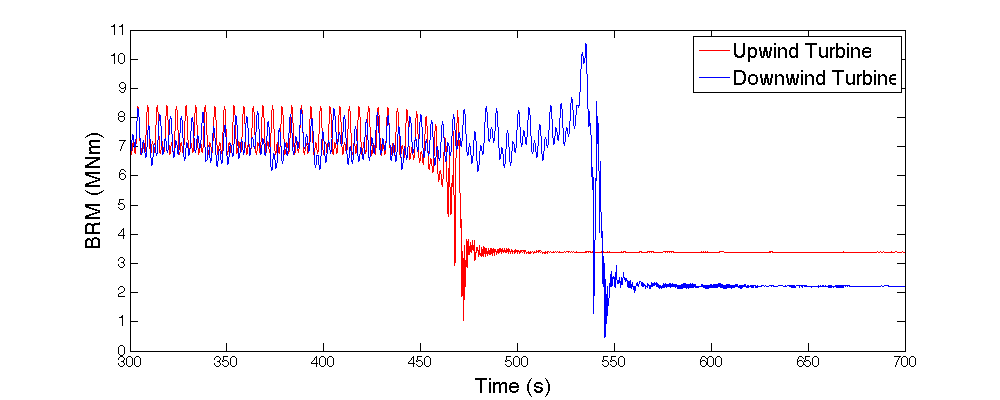
\includegraphics[width = \linewidth]{Figures/ch6Figures/fig6-31.png}

	\caption{Blade root bending moment (BRM) during the Turbine in Wake test case without feed forward control.}
	\label{fig6-31}
\end{figure}

In Figure \ref{fig6-32} we see that the tower base fore-aft bending moments for the upwind turbine is initially constant at approximately 48 MNm. The tower base bending moment is highly dependent on the aerodynamic loading, which is highly dependent on blade pitch. As wind speeds begin to increase and blade pitches begin to increase we see a smooth reduction in tower fore-aft bending moment. The emergency shutdown process causes a short period of cyclical loading, including one large loading cycle where the tower base fore-aft bending moment goes from 47 MNm to -41 MNm. Early in the simulation the downwind turbine has slightly lower tower base fore-aft bending moments, but has more fluctuations in loading. This is due to wake effects. The downwind turbine without feed forward control experiences a sharp increase in loading when the gust arrives at t = ~520 s. As discussed in the previous paragraph, this is because the downwind turbine maintains a 0\degree blade pitch angle until the rotor speed increases to 12.1 RPM. The combination of high wind speed and low blade pitch angle causes very high aerodynamic loading. The emergency shutdown process causes a short period of cyclical loading, including an abrupt change from 76 MNm to -46 MNm. The downwind turbine with Feed Forward Derating Control is derated at t = 478.7 s. This causes a reduction in tower base fore-aft bending moment. This is consistent with a reduction in aerodynamic loading on the turbine rotor due to increasing blade pitch. When the gust arrives loading sharply increases to 63.4 MNm. This brief period of high loading occurs as the turbine transitions from region 2 to region 3 control. By t = 550 s the mean tower fore-aft bending moment has decreased to approximately 2 MNm. However, a cyclic loading component persists through the end of the simulation. If we zoom in on these high frequency oscillations, we see that the loading has a very similar shape to the cyclic BRM loading seen in Figure \ref{fig6-31}, but has a frequency three times higher. Since the turbine rotor has three blades, this indicates that the higher magnitude BRM oscillations seen near the end of the simulation are causing the high frequency oscillations in tower loading. 


\begin{figure}[ht] 
	\centering
		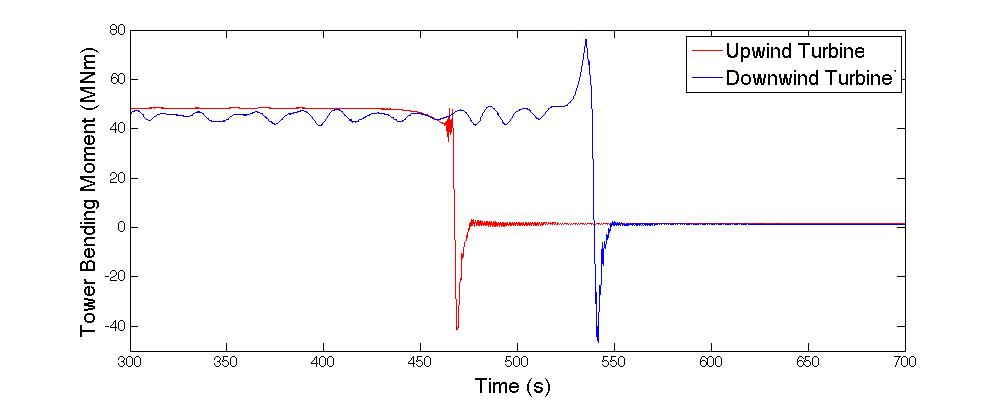
\includegraphics[width = \linewidth]{Figures/ch6Figures/fig6-32.png}

	\caption{Tower base fore-aft bending moment during the Turbine in Wake test case without feed forward control.}
	\label{fig6-32}
\end{figure}


Table \ref{Table6-6} summarizes several important performance metrics for the turbines. The downwind turbine without feed forward control has much higher Damage Equivalent Loads (DEL) than the upwind turbine. If we look at figures \ref{fig6-31} and \ref{fig6-32} it is easy to see where the discrepancy in DEL is coming from. The downwind turbine has much higher loads and more loading fluctuations due to the Extreme Coherent Gust and and the subsequent emergency shutdown. However, I think it's useful to discuss what this means for the turbines and what the root cause of this discrepancy is. This discrepancy means that an Extreme Coherent Gust large enough to cause emergency shutdown is more damaging to a turbine in a wake than to a turbine that is not in a wake. The downwind turbine has to endure the change in wind speed caused by the gust in addition to a change in wind speed due to the upwind turbine shutting down. The upwind turbine is initially operating in 12 m/s wind then experiences a sudden increase of 13 m/s to a 25 m/s wind speed. The downwind turbine is initially operating in an average wind speed of 9.4 m/s then experiences a sudden increase of 15.6 m/s to a 25 m/s wind speed. The upwind turbine and the downwind turbine without feed forward control experience similar maximum overspeeds. Finally, we see that the upwind turbine produces 38.88 KWh more energy than the downwind turbine without feed forward control. The downwind turbine without feed forward control operates for a longer period of time before it experiences an emergency overspeed shutdown. However, as we see in Figure \ref{fig6-29}, it generates less power than the upwind turbine due to wake effects.

Feed Forward Derating Control improves turbine behavior in all four performance metrics. Tower base fore-aft bending moment DEL has been reduced by 58.1 MNm, which is a reduction of 56\%. This is likely because the downwind turbine with feed forward derating control does not experience the very large magnitude loading cycles observed immediately prior to and during emergency shutdown. Blade root bending moment DEL has been reduced by 15\% despite the turbine operating for a longer period of time and enduring a larger quantity of BRM loading cycles. Maximum overspeed has been reduced to 11.7\%, which will not induce an emergency shutdown. Energy generation has been increased by 201.14 KWh.

It is important to note that the difference in energy generation could be much larger in real world operation. These simulations end at t = 700 s, but beyond that time the downwind turbine with feed forward derating control would continue to generate 5 MW (or ~1.4 KWH per second). The downwind turbine without feed forward derating control would not generate any power until it was returned to service. That turbine may be shut down for much longer than the 158.8 seconds captured in these simulations.


\begin{table} [ht]
\centering
\begin{tabular}{c|cccccccccc}
\hline
\hline
                                                                                         &  & \begin{tabular}[c]{@{}c@{}}Tower Base\\ DEL(MNm)\end{tabular} & & \begin{tabular}[c]{@{}c@{}}Blade Root\\ DEL(MNm)\end{tabular} &  & \begin{tabular}[c]{@{}c@{}}Max\\ Overspeed(\%)\end{tabular} &  &  \begin{tabular}[c]{@{}c@{}}Energy\\ Gen.(kWh)\end{tabular}\\ 
\hline
\begin{tabular}[c]{@{}c@{}}Upwind \\ Turbine \end{tabular}                               &  & 76.4                                                          & & 6.92                                                          &  & 16.12                                 				       &  &  233.39                                                    \\
\\
\begin{tabular}[c]{@{}c@{}}Downwind \\ Turbine \\ Without FF \\ Control\end{tabular}     &  & 104.0                                                          & & 9.49                                                          &  & 16.03                                                       &  &  194.51                                                    \\
\\
\begin{tabular}[c]{@{}c@{}}Downwind \\ Turbine \\ With FF \\ Control \end{tabular}       &  & 45.9                                                          & & 8.03                                                          &  & 11.70                                                         &  &  395.65                                                     \\
\\
\begin{tabular}[c]{@{}c@{}}Change   \\ Due to FF \\ Control          \end{tabular}       &  & \begin{tabular}[c]{@{}c@{}}-58.1 \\ (-55.8\%)  \end{tabular}   & & \begin{tabular}[c]{@{}c@{}} -1.46 \\ (-15.4\%)  \end{tabular}   &  & \begin{tabular}[c]{@{}c@{}} -4.33 \\    \end{tabular}        &  &  \begin{tabular}[c]{@{}c@{}}+201.14\\(+103.4\%)\end{tabular} \\
\\
\hline
\hline                             
\end{tabular}
\caption{Summary of turbine performance metrics and the effects of Feed Forward Derating Control for the Turbine in Wake test case.}
\label{Table6-6}
\end{table}


%----------------------------------------------------------------------------------------
%	SECTION 8
%----------------------------------------------------------------------------------------

\section{Conclusions} \label{section6-8}

Chapter \ref{Chapter4} investigated the benefits and feasibility of derating a downwind turbine based on a feed forward signal from an upwind turbine. In that chapter a feed forward derating control scheme was developed and evaluated using a series of FAST simulations. Though the FAST based simulation results were promising, the simulation methodology used to generate them had several noteworthy limitations. The FAST based simulations did not model emergency overspeed shutdowns or turbine to turbine wake effects. Furthermore, the FAST based simulations assumed Taylor's Frozen Turbulence Hypothesis, which provides a very simplistic model of wind speed fluctuations passing through the wind farm.

In this chapter, feed forward derating control was demonstrated and evaluated using a more sophisticated simulation tool that does not have the limitations of the FAST simulations carried out in Chapter \ref{Chapter4}. NREL$'$s Simulator fOr Wind Farm Applications (SOWFA) is a wind farm simulation tool. It uses FAST to model the dynamics of one or more turbines, a Large Eddy Simulation (LES) to model atmospheric airflow, and actuator line models to enable interaction of the LES and FAST models. Because SOWFA models atmospheric airflow, we can run simulations that will capture the evolution of a gust over time, wake effects, and the time it takes a gust to reach the downwind turbine. As we saw in Chapter \ref{Chapter5}, SOWFA can be tuned to provide good agreement with both Reynolds Averaged Navier Stokes (RANS) and FAST simulations of the NREL 5-MW turbine. This adds confidence that our SOWFA simulation results are realistic.

In this chapter the feed forward derating control scheme developed in Chapter \ref{Chapter4} was implemented as a series of FORTRAN subroutines and inserted into the SOWFA source code. Additional control logic was inserted to model emergency overspeed shutdowns (Section \ref{section6-2}). SOWFA$'$s actuator line model was tuned to produce good agreement with FAST. A Gausian projection width of 7.5 produced good agreement across the range of region 3 turbine operation (Section\ref{section6-3}). We discussed the trade offs involved in choosing appropriate computational domain sizes and grid resolutions. Ultimately a near rotor grid resolution of 2 m and a far field resolution of 32 m were chosen. The computational domain size was chosen to be 80R $\times$ 40R $\times$ 40R. (Section \ref{section6-4}). Section \ref{section6-5} discussed gust modeling in SOWFA. The gust was modeled using a mapped fixed value boundary condition on the inlet to the computational domain. Net inflow was held constant by increasing wind speed on some parts of the inlet while decreasing wind speed on other parts. After preliminary simulations an Extreme Coherent Gust (ECG) was chosen instead of the Extreme Operating Gust (EOG) used in Chapter \ref{Chapter4} simulations.

Feed forward derating control was demonstrated and evaluated using two test cases. In the first test case one NREL 5-MW turbine was 20R downwind and 3R offset from another NREL 5-MW turbine. The turbines operated in a constant 12 m/s wind until an Extreme Coherent Gust (ECG) increased wind speed to 25 m/s. Without feed forward derating control the ECG caused emergency overspeed shutdowns of both turbines. Both turbines experienced similar overspeeds and Damage Equivalent Loads (DEL). The downwind turbine produced more energy, but only because it operated longer before the ECG arrived. When the test case was run with feed forward derating control enabled the downwind turbine was able to avoid an emergency overspeed shutdown. Feed forward derating control dramatically reduced the downwind turbine's overspeed and DELs while dramatically increasing power generation.

In the second test case one NREL 5-MW turbine was 20R directly downwind of and in the wake of another NREL 5-MW turbine. As in the previous test case, wind speed is 12 m/s until an Extreme Coherent Gust (ECG) increases wind speed to 25 m/s. In this test case the upwind turbine's wake significantly reduced the power generation of the downwind turbine. Prior to the ECG's arrival the upwind turbine generated 5,000 kW while the downwind turbine produced approximately 44\% less power on average. Without feed forward derating control the ECG caused emergency overspeed shutdowns of both turbines. The downwind turbine experienced much higher Damage Equivalent Loads than the upwind turbine, especially the tower fore-aft bending moment DEL. The downwind turbine produced more energy, but only because it operated longer before the ECG arrived. When the test case was run with feed forward derating control enabled the downwind turbine was able to avoid an emergency overspeed shutdown. Feed forward derating control dramatically reduced the downwind turbine's overspeed and DELs while dramatically increasing power generation.

These test cases illustrate that feed forward derating control can enable a turbine to avoid an emergency shutdown. They also demonstrate that avoiding an emergency shutdown can greatly improve turbine performance by both reducing DELs and increasing power production. The usefulness of feed forward derating control will vary based on site specific conditions, such as how frequent emergency overspeed shutdowns occur. However, it would be very inexpensive to implement because it does not require any sensors that modern turbines don't already have. At a site with favorable conditions, feed forward derating control could provide a significant improvement in performance for a minimal financial investment.